\documentclass[a4paper,12pt]{book}

% Layout
% Gráficos e layout

\ifx\pdfmatch\undefined
\else
    \usepackage[T1]{fontenc}
    \usepackage[utf8]{inputenc}
\fi

% xetex:
\ifx\XeTeXinterchartoks\undefined
\else
    \usepackage{fontspec}
    \defaultfontfeatures{Ligatures=TeX}
\fi

% luatex:
\ifx\directlua\undefined
\else
    \usepackage{fontspec}
\fi

% End engine-specific settings

% Fonte
%\usepackage{lmodern}
\usepackage{times}

% Pacotes adicionados
\usepackage{ae}
% Língua e hifenização
\usepackage[portuguese]{babel}
\usepackage{hyphenat}
\usepackage{hyperref} % Permite Links personalizados
\usepackage{fancyhdr}
\usepackage{sectsty}
\usepackage{float}   % Gerencia melhor o posicionamento das figuras e tabelas
%\usepackage{graphicx}
\usepackage[pdftex]{color,graphicx}
\usepackage{hyperref}
\usepackage{enumerate} % Permite alterar Layout do enumerate
\usepackage{enumitem}  % Permite opções de {itemize}
%\usepackage{pdflscape}  % Permite alterar a orientação da pagina para Paisagem
%\usepackage{ifthen}  % Permite usar condicionais ifelse
\usepackage{xcolor} %cores
\usepackage{amsmath,amssymb} % Ambiente para uso de elementos matemáticos
\usepackage{caption}
\usepackage{subcaption} % permite o uso de multiplas figuras com legenda (ambiente subfigure)
\usepackage{minted} % Ambiente para blocos de código
\usepackage{natbib} % Para referencia bibliográfica
\usepackage{url}    % Referência de links na internet
%\usepackage{listings} % pacote para apresentar código de programação
\usepackage{indentfirst}  % Para indentar o primeiro parágrafo de cada seção
\usepackage{titling}  % Permite Montar uma página de titulo própria
\usepackage{tcolorbox} % Caixas Coloridas com Bordas =D
\usepackage{multicol} % Permite colocar textos e imagens lado a lado

% Layout do documento

% Bordas e tamanho da página
\usepackage{geometry} 
 \geometry{ % Padrõa ABNT para relatórios
 a4paper,
 left=30mm,
 right=20mm,
 top=30mm,
 bottom=20mm
 }

% Cabeçalho e Rodapé
\pagestyle{fancy} % https://www.sharelatex.com/learn/Headers_and_footers
  \lhead{}
  \chead{}
  \rhead{Projeto Edubot} % cabeçalho margem direita
  \lfoot{}
  \cfoot{}
  \rfoot{\thepage} % rodapé margem direita

% Numeração
  \pagenumbering{arabic}

% Retas do cabeçalho e rodapé
  \renewcommand{\headrulewidth}{0.5pt}
  \renewcommand{\footrulewidth}{0.5pt}

% Tamanho da letra
    \chapterfont{\huge}
    \sectionfont{\Large}
    \subsectionfont{\large}

% Hiperlinks
\hypersetup{
    colorlinks,
    citecolor=black,
    filecolor=black,
    linkcolor=black,
    urlcolor=black
}

% Definições do pdf
\hypersetup{
    unicode=false,          % non-Latin characters in Acrobat’s bookmarks
    pdftoolbar=true,        % show Acrobat’s toolbar?
    pdfmenubar=true,        % show Acrobat’s menu?
    pdffitwindow=false,     % window fit to page when opened
    pdfstartview={FitH},    % fits the width of the page to the window    
    pdfauthor={Projeto Edubot - UnB},     % author
    pdfnewwindow=true      % links in new window
}

% Outros
%\renewcommand{\thesection}{(\alph{section})} % muda o estilo de númeração das sections
% alterando a formatação dos numeradores de lista de itens
\renewcommand\theenumi{\arabic{enumi}}
\renewcommand\labelenumi{\textbf{\alph{enumi})}}
\renewcommand\theenumii{\arabic{enumii}}
\renewcommand\labelenumii{(\textit{\theenumi.\theenumii})}

% Blocos de questões
%   referência:
%   https://tex.stackexchange.com/questions/66154/how-to-construct-a-coloured-box-with-rounded-corners#66156
% Contador para enumerar as questões
\newcounter{question}[subsection]
% Define caixas para formatação
\newtcolorbox{questionbox}[1]{
    colback=blue!5!white, 
    colframe=blue!75!black,
    fonttitle=\bfseries,
    title=#1
}
\newtcolorbox{chalengebox}[1]{
    colback=red!5!white,
    colframe=red!75!black,
    fonttitle=\bfseries,
    title=#1
}
% Formatar questões
\newcommand{\question}[1]{\stepcounter{question}\noindent
\begin{questionbox}{Exercício \thesection.\thequestion\hspace{0.2cm}}
#1
\end{questionbox}}
% Formatar questões de desafio mantendo a numeração
\newcommand{\challenge}[1]{\stepcounter{question}\noindent
\begin{chalengebox}{\thesection.\thequestion\hspace{0.2cm} Desafio}
#1
\end{chalengebox}}
\newcommand{\FNada}[1]{#1}

\def\BibTeX{{\rm B\kern-.05em{\sc i\kern-.025em b}\kern-.08em
    T\kern-.1667em\lower.7ex\hbox{E}\kern-.125emX}}
% permite que o comando \underline{\hspace{.1in}} escreva um underline

\usepackage[document]{ragged2e}


\title{Apostila didática}
\author{Projeto Edubot}

\begin{document}
% Capa da apostila
\begin{figure}[h!]
    \centering
    
\includegraphics[scale=0.9]{Figuras/simb_unb.png}
    \label{fig:unb}
    \caption*{Universidade de Brasília}
\end{figure}

\begin{center}
    Departamento de Engenharia Elétrica
    
    Capitulo Estudantil IEEE de Robótica e Automação (IEEE - RAS UnB)
    
    Projeto Edubot
    
    \vfill
    
    \Huge \bf \thetitle
    
    \vfill
    
    \large % fonte
    
    Brasília \\
    \the\year % Coloca o Ano atual
    
    \thispagestyle{empty} % Retira o cabeçalho e o rodapé da página
\end{center}

% Cabeçalho
\newpage
Incluir aqui um cabeçalho para o aluno preencher seu nome, sua escola e alguns dados pessoais.
\tableofcontents
\newpage


\chapter*{Como usar esta apostila?}
   Explicar o objetivo da apostila para qualquer pessoa que pegar ela para ler. Além disso, explicar aos alunos como devem utilizá-la ao longo de seus estudos.

\chapter{Afinal, o que é um robô?}
\section*{Introdução}
\paragraph{}
O desejo de solucionar problemas do dia-a-dia de maneira mais eficiente e simples, foi - e ainda é - um dos maiores promotores para o desenvolvimento tecnológico das mais diversas sociedades. De acordo com a necessidade de cada período, cientistas (engenheiros, matemáticos, físicos, etc) de diferentes povos propunham maquinários e ferramentas que pudessem operar em conjunto com outros seres vivos para \textbf{modificar} a forma de trabalho, melhorando a qualidade de vida dos trabalhadores e das suas famílias. Com isso, impulsionou-se a busca por maiores níveis de \textbf{automação}, consequentemente levando às tentativas de aplicar esse conceito no cotidiano, sendo esse o patamar que alcançamos e presenciamos nos dias atuais.\\

É nesse contexto que a ideia da utilização de robôs para a realização de diversas tarefas acabou se popularizando, colocar uma máquina para completar uma tarefa muito trabalhosa ou difícil e assim poupar trabalho humano é um dos focos da robótica. O robozinho utilizado como material de estudo no nosso curso é o \textit{Sparki}, ele é uma dessas máquinas que tem como objetivo facilitar a nossa vida, nesse caso o ensino de programação, mas o que difere ele e outros robôs de um ar condicionado ou um projetor? \par

\section{Para que estudar a definição de robô?}

\paragraph{}
Como descrito na introdução desse capítulo, a robótica está presente em diversos aspectos do nosso cotidiano. Dentre as mais diversas aplicações existentes, podemos listar algumas:

\begin{itemize}
\item Culinária, robôs que auxiliam na preparação de pratos e na entrega dos mesmos em restaurantes (segue-linha);

\item Robôs industriais, como carregados (segue-linha), robôs montadores de peças em indústrias;

\item Robôs cirúrgicos, como o Star (tecidos moles mais delicados), o PRECEYES (áreas delicadas, como os olhos), CorPath (operações cirúrgicas a distância através do Wifi), The Monarch Platform (broncoscopia, i.e. intervenção cirúrgica nos brônquios), Mako Rio (auxiliar em implante em joelhos e costela), Versius (cirurgias não invasivas);

\item Robôs para comunicação com crianças;

\item Robôs de exploração espacial, como o Hover em Marte;

\item Robô para inspecionar de tubulações;

\item Robô para serviços de casa (seja de superfícies aquáticas, ou terrestres). Exemplos: Row-bot, Ro-Boat, Roomba.
\end{itemize}

    \begin{figure}[h]
    \caption{Exemplo de um robô, o Roomba}
     
    \centering 
    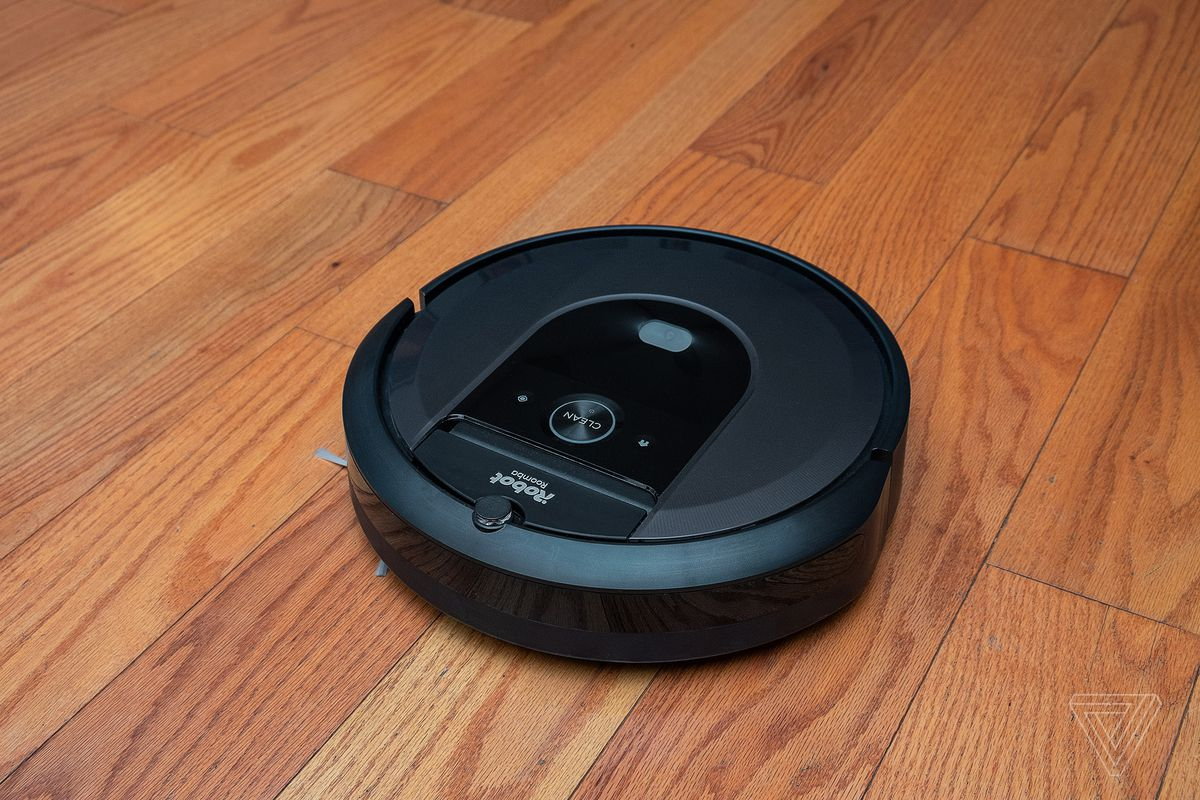
\includegraphics[width=8cm]{Figuras/roomba.jpg}
    \label{figura:roomba.jpeg}
    \end{figure}
 

\section{Definindo um robô}
\paragraph{}
Para uma máquina ser considerada um robô, a primeira coisa que ela deve ser capaz de fazer é raciocinar de alguma maneira.\\

\textit{Como assim, um robô tem que ser capaz de pensar assim como nós (pessoas)?} \par
Não necessariamente, algo assim é muito complexo e difícil de acontecer... Quando dizemos que um robô deve raciocinar, queremos dizer que ele deve ter a capacidade de analisar o mundo ao seu redor e tomar decisões a partir do que ele analisou, ele precisa agir em função do seu ambiente. Um robô segue linhas por exemplo, necessita de algum sensor que permita a ele encontrar a localização da linha e a partir dai decidir como irá se movimentar sobre ela e o que fazer caso perca a linha de vista. De maneira geral, a ação realizada pelos robôs normalmente é algum tipo de movimento, alguma atividade mecânica como andar ou mover algo, um semáforo que acende a luz vermelha para os carros para possibilitar a passagem de pedestres após ter seu botão apertado não é considerado um robô, uma porta automática de um shopping se aproximaria mais do que é um robô.\\

\textit{Qual a relevância deste assunto no mundo? Afinal, para que mesmo eu estou lendo esta apostila? Eu sei que eu vou ganhar um diploma do curso, mas... E aí? O que mais que isso aqui pode me acrescentar?}\par
Nosso curso busca ajudar os alunos a entender de forma simples como que um robô, um computador ou outros equipamentos raciocinam, como que nós pessoas somos capazes de criar linhas de pensamento para coisas não pensantes. Nós mostraremos que a programação não é um bicho de sete cabeças e forneceremos a base necessária para que vocês cheguem mais preparados e entusiasmados em algum curso superior, técnico ou trabalho que aborde programação.

\begin{center}

    \textbf{Definição}
    
    \justify
    Um robô é uma máquina \textbf{autônoma}, que existe no \textbf{mundo físico}, possui \textbf{sensores} para perceber o ambiente e consegue \textbf{agir} sobre o meio para alcançar um ou mais objetivos definidos.
\end{center}

\paragraph{}
Nós já falamos sobre os sensores e conseguir agir sobre o meio, mas e os outros requisitos?
Existir no mundo físico nada mais é do que algo que somos capazes de tocar e manipular, uma bola de futebol por exemplo existe no mundo físico, os sonhos que temos ao dormir não existem no mundo físico, pois não somos capazes de tocá-lo.
Uma máquina autônoma ou automática, é uma máquina que após ligada ela funciona sozinha sem a constante necessidade de interferência externa, ela ainda pode aceitar o aperto de botões ou o recebimento de outros tipos de comandos, mas a ideia é que ela seja capaz de realizar tarefas sozinha quando for necessário.

\section*{Para saber mais}

\begin{enumerate}
    \item Mais informações sobre o sistema robótico PRECEYES estão disponíveis em:

    \url{https://www.brabantbrandbox.com/life-sciences/preceyes/}. Acesso em 13 de Agosto de 2019.
    
    \item Quer saber um pouco mais sobre os procedimentos cardíacos auxiliados pelo CorPath? Acesse: https://www.corindus.com/
    \item Mais informações sobre The Monarc Plataform em:


    https://www.aurishealth.com/monarch-platform.
    \item Mais informações sobre o Mako Rio em: \\
    \url{https://www.stryker.com/us/en/portfolios/orthopaedics/joint-replacement/mako}
    \url{-robotic-arm-assisted-surgery.html}.
    \item Assista o próprio Jonathan Rossiter falando sobre o Rowbot em:
    
    \url{https://www.youtube.com/watch?v=KCL8NjN7FMQ}.
    
    \item Mais informações sobre o Ro-boat em:
    http://roboat.org/.
    \item Introdução à robótica - Maja Mataric. \\
    \url{https://web.icmc.usp.br/SCATUSU/Boletim_aquisicao/Boletim_novembro_2016/Capas_novembro_2016/Mataric_Introducao0001.pdf}
\end{enumerate}

\section{Exercícios}

\question{Além das aplicações citadas nesse capítulo, pesquise mais 3 áreas em que a robótica está presente.}

\begin{center}
    \line(1,0){450}
    \vspace{0.2cm}   
    \line(1,0){450}
    \vspace{0.2cm}   
    \line(1,0){450}
    \vspace{0.2cm}   
    \line(1,0){450}
    \vspace{0.2cm}   
\end{center}

\question{Um termômetro pode ser considerado um robô dentro da definição vista neste capítulo? Justifique.}

\begin{center}
    \line(1,0){450}
    \vspace{0.2cm}   
    \line(1,0){450}
    \vspace{0.2cm}   
    \line(1,0){450}
    \vspace{0.2cm}   
\end{center}

\question{Cite 3 exemplos de robôs dentro da cultura popular (filmes, séries, \textit{animes} etc.) que são erroneamente considerados robôs.}

\begin{center}
    \line(1,0){450}
    \vspace{0.2cm}   
    \line(1,0){450}
    \vspace{0.2cm}
\end{center}

\question{Dentre os aparelhos eletrônicos presentes em sua casa, quais deles mais se assemelha às características que definem um robô?}

\begin{center}
    \line(1,0){450}
    \vspace{0.2cm}   
    \line(1,0){450}
    \vspace{0.2cm} 
\end{center}

\challenge{
    {\large{Desafio:}} Escolha algum dos exemplos de robôs apresentados ou algum outro do seu interesse e procure entender a lógica de seu funcionamento (quais os seus sensores, qual a lógica por trás de suas ações).
}

\begin{center}
    \line(1,0){450}
    \vspace{0.2cm}   
    \line(1,0){450}
    \vspace{0.2cm}   
    \line(1,0){450}
    \vspace{0.2cm}   
    \line(1,0){450}
    \vspace{0.2cm}   
\end{center}
\chapter{Algoritmos e tela LCD}
\section*{Introdução}
    Neste capítulo veremos o que significa algoritmo, o que é uma tela LCD e para que ela serve. Além disso, vamos abordar o conceito de linguagem de programação e saber, afinal, como nos comunicar com o \textit{Sparki}. E aí, vamos nessa?
\section{Algoritmo}
    Diariamente utilizamos algoritmos sem mesmo perceber. Quando cozinhamos um macarrão, assamos um bolo, montamos um móvel, um brinquedo ou mesmo quando escovamos os dentes estamos utilizando este conceito para completar essas tarefas. \par
    Isto porque tomamos essas decisões nos baseando em instruções claras para chegar a um objetivo. Então, se estamos preparando um bolo, não podemos simplesmente colocar os ingredientes no forno sem antes misturá-los conforme a receita. Não teríamos um bolo, mas um Frankestein! Da mesma forma, não poderíamos esperar que ele fique pronto se ligarmos o forno, mas não colocássemos a massa do bolo nele. \par
    \begin{center}
    \textbf{Definição} \\
    Algoritmo é um conjunto finito de instruções sequenciais lógicas, bem definidas, não ambíguas que levam à solução de um problema.
    \end{center}
    \textit{Mas afinal o que esse bando de palavras complicadas querem dizer ? Eu não entendi foi nada.}
    
    O que elas querem dizer é, em outras palavras, que um algoritmo indica um conjunto de instruções para realizar uma tarefa qualquer, como por exemplo, fazer pipoca. Seguimos uma receita que nos diz bem direitinho o que fazer para atingir o objetivo desejado, que no caso é aquela pipoca bem quentinha e crocante no final das contas! Assim ficou mais fácil de entender, né? \par
    Como já vimos, robôs não raciocinam como nós, seres humanos. Então precisamos deixar bem claro o que esperamos de cada um deles quando estamos nos comunicamos com eles para que o objetivo final seja cumprido. 
    
    \textit{Ué, mas isto parece exatamente com algo que você já disse.}  
    
    Exatamente! Escrevemos algoritmos para fazer a programação de robôs! \par 
    Até agora vimos que algoritmos são extremamente importantes e é essencial que o seu conceito seja entendido. Mas você sabia que não precisamos de um computador para programar?
\subsection{Torre de copos}
    Desafio torre de copos.


\section{Linguagem de programação}
    Se fosse dado o comando abaixo para o \textit{Sparki} você acha que ele entenderia? \par
    \begin{center}
    \textit{Sparki vai para frente! Sparki vai para trás!}\ \par
    \end{center} \par
    Quem pensou que ele não entenderia acertou, o \textit{Sparki} não iria entender nada do que foi dito. \par
    \textit{Então como ele entende os comandos que pedimos para ele fazer?}\par
    Para nos comunicarmos com o \textit{Sparki}, é preciso passar os comandos para o computador através de uma linguagem de programação, que irá converter o que escrevemos para zeros e uns e depois enviará para \textit{Sparki}, e assim ele será capaz de entender e executar o comando.
    
    \begin{center}
    \textbf{Definição} \\
    Uma linguagem de programação é um método padronizado para comunicar instruções para um computador.
    \end{center} \par
    
 
\subsection{Funções importantes: \textit{void setup(), void loop()}}
    
    A biblioteca  \textit{sparki.h} e as funções \textit{void setup e void loop} são as funções mais importantes na hora de começar a programar o \textit{Sparki}, pois entender o que elas significam e como funcionam é essencial para saber onde escrever determinada parte do código em relação ao tipo de aplicação.
    
    \begin{minted}{cpp}
    #include <Sparki.h>
    void setup()
    {
    }
    void loop()
    {
    }
    \end{minted}

    \begin{itemize}
        \item Biblioteca \textit{sparki.h}: Esta biblioteca guarda todas as funções relacionadas ao \textit{Sparki}, e é necessário inserir ela na primeira linha de código, para que estas funções sejam habilitadas para a comunicação entre o computador e o robô funcionar.
        \item \textit{Void Setup()}: Esta função é a primeira a rodar no código, e tudo que está dentro de suas chaves é executado apenas uma vez. A função é bastante útil para inserir configurações iniciais, como por exemplo limpar a tela LCD, ou fazer algum movimento inicial que não irá se repetir no resto do programa.
        \item \textit{Void Loop}: Esta função é usada para colocar códigos que irão ficar se repetindo no programa, ou seja, sempre ficará rodando até que seja carregado algum outro programa no \textit{Sparki}. Um exemplo para esta função é deixar o \textit{Sparki} sempre com o LED de uma cor ligado, ou sempre se movimentando em uma determinada direção.
        \end{itemize}
    
  %  Escrever código de como mostrar algo na tela do Sparki

\section{Tela de LCD (\textit{Liquid Crystal Display})}
O \textit{Sparki} possui uma tela LCD onde é possível desenhar, escrever e visualizar dados de sensores em funcionamento. A tela é formada por \textit{pixels}, que são pequenos pontos de luz que podem estar ligados ou desligados para formar uma imagem. No caso do \textit{Sparki}, ele possui 128 \textit{pixels} na horizontal e 64 \textit{pixels} na vertical, e para identificar cada pixel deve ser fornecido a coordenada horizontal, vertical, e se ele deverá ficar aceso ou apagado. \par
\textit{Então toda vez que eu for escrever algo no LCD preciso fazer a coordenada de cada pixel?}
Não, porque alguém já disse ao computador como ligar e desligar pixels para formar os caracteres, ou seja, se você quer escrever uma letra 'A' por exemplo, já está armazenado quais pixels devem acender e apagar para que a tela mostre exatamente a letra 'A'.

\section{Exercícios}
\question{Em suas palavras, defina o que é uma linguagem de programação.}
    Deixar espaço de linhas.
    \vspace{4cm}        % Espaçamento vertical
    
\question{O objetivo de uma linguagem de programação é:}
    \begin{enumerate}
        \item Fornecer um conjunto de regras bem definidas que permita escrever programas de computador de forma mais amigável evitando ambiguidades.
        \item Dar a liberdade para cada programador escrever programas de computador a partir do seu próprio conjunto de regras, facilitando o processo de programação.
        \item Estabelecer regras para comunicação entre seres humanos.
        \item Definir um padrão para programadores utilizarem os comandos binários intrínsecos a cada arquitetura de processador.
    \end{enumerate}

\subsection{}

\subsection{}

\subsection{}

\subsection{\large{Desafio:}}
% Capítulo Movimentação =========================================
\chapter{Movimentação}
\section*{Introdução}
    \paragraph{}
    Será neste capítulo que iremos aprender a movimentar o \textsl{Sparki}, os comandos para ele ir para frente, rotacionar e realizar todos os percursos que a nossa imaginação puder criar. Para isso, será necessário utilizar as funções a seguir.
    
\section{Funções}
    \paragraph{}
    Todas as funções desse capítulo começam com \mintinline{cpp}{sparki.move}, você consegue pensar em um motivo para a palavra ``move'' estar em destaque?
    \\~\\
    \textit{Move... Mover... Movimentar...}
    
    Exatamente! Movimentação é a resposta, pois ``move'' significa ``se movimentar'' em inglês.
    
\subsection{sparki.moveForward(int distancia);}
    \paragraph{}
    Essa é a principal função de movimentação, pois é um comando para o robô ``andar'' para frente. Sendo ``distancia'' uma variável que representa quantos centímetros o \textsl{Sparki} deverá se movimentar para frente. Após ter percorrido essa distância, ele passará a executar a próxima linha de comando, ou seja, a próxima ação.
    \\~\\
    \textit{Variável? Mas o que é essa tal de variável?} \\
    Não se preocupe! Teremos um capítulo inteiro apenas para entendê-la, mas, por enquanto, iremos utilizá-la para informar ao \textsl{Sparki} qual a distância em centímetros que queremos que ele percorra. Simples assim!
    \\~\\
    \textit{E o que significa esse `int' dentro dos parênteses?} \\
    Ele indica que o número que colocaremos dentro dos parênteses tem que ser um número inteiro.
    
    \begin{center}
    \textcolor{teal}{Lembrando:} Números inteiros são aqueles que não têm a parte decimal, ou seja, não possuem vírgula. $\mathbb{Z}=\{..., -3, -2, -1, 0, 1, 2, 3, ...\}$.
    \end{center}
    
    \paragraph{}
    Como queremos que o \textsl{Sparki} vá para frente, além de ser um número inteiro, tem que ser positivo também! Ah! Se não tiver escrito nada no espaço entre os parênteses, o \textsl{Sparki} irá para frente indefinidamente, ou seja, até que seja lida a função \mintinline{cpp}{sparki.moveStop()}, ou até que a bateria dele acabe...
    \paragraph{}
    Parece complicado, mas vou dar um exemplo passo a passo para você ver que não é.
    \\~\\
    \textsc{Exemplo 1)} Vamos supor que o seu objetivo é fazer o \textsl{Sparki} andar para frente.
    
    \begin{itemize}
        \item O primeiro passo é identificar a função a ser utilizada para o \textsl{Sparki} andar para frente, neste caso, \mintinline{cpp}{sparki.moveForward(int distancia)};
        \item O segundo passo é decidir o qual vai ser o valor a ser escrito entre os parênteses, ou seja, o parâmetro dessa função. Como não determinamos uma distância, pois queremos que ele ande para frente e não pare, não é necessário escrever um número, basta deixar em branco;
        \item Agora que sabemos a função e o seu parâmetro, podemos aplicar no código. Ficaria assim:
    \end{itemize}
    
    \begin{minted}{cpp}
    #include <Sparki.h>
    void setup()
    {
    }
    void loop()
    {
        sparki.moveForward();
    }
    \end{minted}
    
    \paragraph{}
    Quando queremos passar uma informação para outra pessoa, podemos falar de diversas formas, seja de um jeito mais devagar ou até muito rápido, bem formal ou com várias gírias. Então, pode-se dizer que, independente do modo com que falamos, a pessoa irá entender a informação, mas, dependendo da pessoa com quem falamos, devemos escolher o modo mais conveniente. Por exemplo, não podemos falar da mesma forma com os nossos amigos e com o/a diretor/a do colégio, para este último devemos tentar utilizar uma linguagem mais formal. Na programação isso também acontece, existem vários códigos diferentes que fazem basicamente a mesma coisa, mas sempre devemos escolher o mais eficiente ou conveniente para cada caso.
    \\~\\
    \textsc{Exemplo 2)} Vamos aproveitar para ver um código que faz o mesmo que o do \textsc{Exemplo 1}. Outra forma de fazer o robô andar para frente sem parar seria escrevendo um número qualquer como parâmetro \mintinline{cpp}{sparki.moveForward(int distancia)}.
    
    \begin{minted}{cpp}
    #include <Sparki.h>
    void setup()
    {
    }
    void loop()
    {
        sparki.moveForward(100);
    }
    \end{minted}
    
    \textit{Como assim?? Você disse que o número que vinha dentro dos parênteses determinava a distância. Então, se eu colocar um número qualquer, o \textsl{Sparki} vai parar depois de andar a distância escrita, não?} \\
    Sim, o número dentro dos parênteses indica sim a distância a ser percorrida, mas há algo que você pode estar se esquecendo. Tente se lembrar da definição de \mintinline{cpp}{void loop()}. Ela falava que tudo o que estiver escrito dentro das chaves do \mintinline{cpp}{void loop()} seria repetido várias e várias vezes, até que a bateria do robô acabe. Como só existe uma função dentro do loop, essa vai se repetir para sempre, é como se o \textsl{Sparki} estivesse andando 100 centímetros para frente e, depois que terminasse, mais 100 centímetros para frente e depois mais 100 centímetros para frente... Essa sequência ficaria se repetindo, sem parar.
    
    \paragraph{}
    Bom, chegamos a conclusão de que o \textsc{Exemplo 1} e o \textsc{Exemplo 2} são códigos que geram a mesma ação, agora devemos pensar em qual seria mais eficiente ou conveniente na hora de escrever. Geralmente, optamos pelo código mais simples, sem elementos desnecessários, para que quem estiver lendo possa compreender melhor o nosso código. Logo, o \textsc{Exemplo 1} seria a melhor escolha.
    
    \begin{center}
    \textcolor{cyan}{Para não esquecer!} \\``Forward'' traduzido para o português significa ``para frente''. 
    \\Assim ficou fácil de lembrar, não é mesmo?
    \end{center}

\subsection{sparki.moveBackward(int distancia);}
    \paragraph{}
    Parecida com a anterior, essa função é utilizada para que o \textsl{Sparki} ``ande'' para trás, sem fazer giros. Sendo ``distancia'' uma variável que representa quantos centímetros ele deverá se movimentar para trás. Da mesma forma que o \mintinline{cpp}{sparki.moveForward()}, se não for escrito nada no espaço entre os parênteses, o \textsl{Sparki} irá para trás indefinidamente, ou seja, até que seja lida a função \mintinline{cpp}{sparki.moveStop()}.
    \\~\\
    
    \textsc{Exemplo 1)} Nesse exemplo, veremos um código que faz o \textsl{Sparki} andar 1 metro para frente e 1 metro para trás.
    
    \begin{itemize}
        \item As funções necessárias são: \mintinline{cpp}{sparki.moveForward(int distancia)}, para andar para frente, e \mintinline{cpp}{sparki.moveBackward(int distancia)}, para andar para trás;
        \item A distância é de 1 metro, mas como o valor tem que ser em centímetro, devemos transformar de metro para centímetros. Substituindo os parâmetros, as funções ficariam assim: \mintinline{cpp}{sparki.moveForward(100)}, \mintinline{cpp}{sparki.moveBackward(100)}.
        \item Agora é só escrever em forma de código!
    \end{itemize}
    
    \begin{minted}{cpp}
    #include <Sparki.h>
    void setup()
    {
    }
    void loop()
    {
        sparki.moveForward(100);
        sparki.moveBackward(100);
    }
    \end{minted}
    
    Também poderíamos inserir a função \mintinline{cpp}{delay(int tempo)} entre as funções de movimentação para que o \textsl{Sparki} realize melhor esses movimentos.
    \\~\\
    \textit{O que essa função delay(int tempo) faz mesmo?} \\
    Ela estabelece um tempo de intervalo entre as ações, simplificando, o \textsl{Sparki} espera um tempo determinado pela variável ``tempo'' antes de executar a próxima ação, com isso, podemos acompanhar melhor a execução dos movimentos que escrevemos no nosso código.
    \\~\\
    \textsc{Exemplo 2)} Agora, iremos reescrever o código anterior utilizando a função \mintinline{cpp}{delay(int tempo)} para que, antes do \textsl{Sparki} mudar o sentido do seu movimento, ele dê uma pausa de 3 segundos.
    
    \begin{minted}{cpp}
    #include <Sparki.h>
    void setup()
    {
    }
    void loop()
    {
        sparki.moveForward(100);
        delay(3000);
        sparki.moveBackward(100);
        delay(3000);
    }
    \end{minted}
    
    \textit{Por que existem dois \mintinline{cpp}{delay(3000)} no código?}
    
    O primeiro é necessário para estabelecer um intervalo entre andar para frente e andar para trás. O segundo serve para estabelecer um intervalo entre andar para trás e andar para frente, porque, como as funções estão dentro do \mintinline{cpp}{void loop}, depois de \mintinline{cpp}{sparki.moveBackward(100)} o próximo movimento seria \mintinline{cpp}{sparki.moveForward(100)}, então, devemos colocar uma pausa ali também.  
    
    \begin{center}
        \textcolor{teal}{Lembrando:} No exemplo anterior nós utilizamos a palavra ``sentido'' no enunciado. Mas você se lembra o que realmente significa esse conceito? E qual a diferença entre ``sentido'' e ``direção''? Vou dar um exemplo para você não errar mais na hora de diferenciar os dois.
    \end{center}
    
    \paragraph{}
    Vamos supor que você saiu de casa e ficou perdido no meio da cidade apenas com a sua pulseira da sorte e uma bússola para te auxiliar a voltar para casa. Essa bússola vai indicar a direção sul, norte, leste, oeste e as várias direções de acordo com os 360 graus dela. Você tem o conhecimento de que a sua casa fica para o sul, por isso, começa a andar nessa direção, saindo da cidade e indo para sua casa. Alguns minutos depois você chega ao seu destino, mas percebe que a sua pulseira caiu no meio do caminho. Então você decide ir de novo para a cidade, pela mesma direção que você veio na volta, mas no sentido contrário ao que você utilizou para voltar para casa, ou seja, saindo da sua casa e indo para a cidade. 
    \paragraph{}
    Contada a história, vamos refletir. A direção pode ser simplificada como uma reta que liga a cidade à sua casa e esta reta possui dois sentidos, o de ida e o de volta. Então, quando estamos falando de uma direção, para facilitar, imagine uma linha tracejada entre o local inicial e o seu ponto de destino. Quando estamos falando de sentidos, pense nessa linha como uma seta (casa -> cidade) para a ida e (cidade -> casa) para a volta.

    \begin{center}
    \textcolor{cyan}{Para não esquecer!} \\ ``Backward'' traduzido para o português significa "para trás".
    \end{center}
    
    
\subsection{sparki.moveStop();}
    \paragraph{}
    Esse é um comando para o \textsl{Sparki} parar de se movimentar, independente do que ele estiver fazendo. Observe que não é necessário escrever nada dentro dos parênteses, o robô irá parar de realizar a ação que ele estiver fazendo no momento em que esse comando for lido.
    
    \begin{center}
        \textcolor{teal}{Lembrando:} O tempo a ser escrito como parâmetro, dentro dos parênteses, deve estar em milissegundos.
    \end{center}
    \\~\\
    \textsc{Exemplo 1)} Neste próximo exemplo, faremos o \textsl{Sparki} andar para frente por 2 segundos e parar, repetidamente.
    
    \begin{itemize}
        \item Primeiro vamos identificar as funções a serem utilizadas para o \textsl{Sparki} andar para frente, esperar 2 segundos e parar. Como vimos no exemplo anterior, a função \mintinline{cpp}{sparki.moveForward(int distancia)} será responsável por andar para frente. Para esperar 2 segundos, devemos utilizar a função \mintinline{cpp}{delay(int tempo)}. Por último, utilizaremos a função \mintinline{cpp}{sparki.moveStop()}, com o objetivo de fazer o \textsl{Sparki} parar.
        \item Agora, vamos decidir os parâmetros dessas 3 funções. Como queremos que o robô ande durante 2 segundos, a função \mintinline{cpp}{sparki.moveForward(int distancia)} será escrita antes da \mintinline{cpp}{sparki.moveStop()}. O \textsl{Sparki} deverá andar por 2 segundos, logo, essa função deverá ser escrita entre as duas anteriores.
        \item Aplicando em código temos:
    \end{itemize}
    
    \begin{minted}{cpp}
    #include <Sparki.h>
    void setup()
    {
    }
    void loop()
    {
        sparki.moveForward();
        delay(2000);
        sparki.moveStop();
    }
    \end{minted}
    
    O uso da função \mintinline{cpp}{delay(int tempo)} é de suma importância para o movimento funcionar, sem ela, as funções de andar para frente e parar entrarão em conflito.
    
    \begin{center}
    \textcolor{cyan}{Para não esquecer!}
    \\``Stop'' traduzido para o português significa ``Parar''.
    \end{center}
    
\subsection{sparki.moveRight(int graus);}
    \paragraph{}
    Um pouco diferente dos anteriores, esse é um comando de girar para a direita. Sendo ``graus'' uma variável que representa a variação em graus do giro. Se este campo ficar em branco, o \textsl{Sparki} executará um giro de 90° para a direita.
    \\~\\
    
    \textsc{Exemplo 1)} Neste código, o \textsl{Sparki} executará um giro à direita de 90° e ficará parado por 1 segundo antes de executar novamente o giro.
    
    \begin{itemize}
        \item As funções necessárias são: \mintinline{cpp}{sparki.moveRight(int graus)} para girar para a direita e \mintinline{cpp}{delay(int tempo)} para gerar uma pausa;
        \item Substituindo os parâmetros, as funções ficariam assim: \mintinline{cpp}{sparki.moveRight()}, pois 90° é o mesmo que deixar em branco, e \mintinline{cpp}{delay(1000)}.
        \item Escrevendo em forma de código:
    \end{itemize}
    
    \begin{minted}{cpp}
    #include <Sparki.h>
    void setup()
    {
    }
    void loop()
    {
        sparki.moveRight();
        delay(1000);
    }
    \end{minted}
    
    \begin{center}
    \textcolor{cyan}{Para não esquecer!}
    \\``Right'' traduzido para o português significa ``Direita'', mas lembre-se que não é um deslocamento para direita, e sim um giro.
    \end{center}
    
\subsection{sparki.moveLeft(int graus);}
    \paragraph{}
    Esta função é responsável pelo giro para a esquerda do \textsl{Sparki}. Sendo ``graus'' uma variável que representa a variação em graus do giro. Se este campo ficar em branco, o \textsl{Sparki} executará um giro de 90° para a esquerda.
    \\~\\
    \textsc{Exemplo 1)} Neste exemplo, nós criaremos um código que fará o \textsl{Sparki} realizar um giro completo para a direita, esperar 1 segundo, realizar um giro completo para a esquerda e esperar mais 1 segundo antes que ele repita a sequência.
    
    \begin{itemize}
        \item As funções necessárias são: \mintinline{cpp}{sparki.moveRight(int graus)} para girar para a direita, \mintinline{cpp}{sparki.moveLeft(int tempo)} para girar para a esquerda, além da \mintinline{cpp}{delay(int tempo)} para o intervalo;
        \item Para completar um giro, é necessário realizar os 360 graus, por isso, esse número deve ser escrito dentro dos parênteses das funções de girar. Com o objetivo de fazer uma pausa de 1 segundo, devemos escrever 1000 dentro dos parênteses da função de pausa. Substituindo os parâmetros, as funções ficariam assim: \mintinline{cpp}{sparki.moveRight(360)}, \mintinline{cpp}{sparki.moveLeft(360)}, \mintinline{cpp}{delay(1000)}.
        \item Escrevendo em forma de código:
    \end{itemize}
    
    \begin{minted}{cpp}
    #include <Sparki.h>
    void setup()
    {
    }
    void loop()
    {
        sparki.moveRight(360);
        delay(1000);
        sparki.moveLeft(360);
        delay(1000)
    }
    \end{minted}
    \\
    \textsc{Exemplo 2)} Que tal juntarmos a função de andar para frente e girar para a esquerda? O código a seguir faz \textsl{Sparki} ir e voltar em uma linha reta. Os movimentos passo a passo são os seguintes: ir para frente por 0,1 metro, esperar 1 segundo parado, girar para a esquerda 180 graus e esperar 1 segundo parado antes de repetir.

    \begin{minted}{cpp}
    #include <Sparki.h>
    void setup()
    {
    }
    void loop()
    {
        sparki.moveForward(10);
        delay(1000);
        sparki.moveLeft(180);
        delay(1000)
    }
    \end{minted}
    \begin{center}
    
   \textcolor{cyan}{Para não esquecer!}
   \\``Left'' traduzido para o português significa ``Esquerda'', mas lembre-se que não é um deslocamento para esquerda e sim um giro.
    \end{center}
    
\subsection{sparki.motorRotate(int motor, int direcao,  int velocidade);}

Quer aprofundar um pouco mais o seu conhecimento sobre movimentação? Então vamos nessa!
\paragraph{}
Sabemos que o \textsl{Sparki} possui duas rodas, mas, para que elas possam rotacionar e fazer o robô se movimentar, tem que existir algo gerando um movimento de rotação. E quem se ocupa dessa tarefa é o motor. Como são duas rodas, existem dois motores, um do lado de cada roda. Para padronizar, iremos chamar o motor do lado direito de ``MOTOR\_RIGHT'' e o motor do lado esquerdo de ``MOTOR\_LEFT''. Agora já sabemos que tem um motor para gerar o movimento, mas, além disso, é necessário decidimos mais duas coisas: qual será a direção para onde ele irá girar e qual será a velocidade dessa rotação. Exitem duas direções de rotação, uma seria o sentido horário e outra o sentido anti-horário, elas serão chamadas respectivamente de: ``DIR\_CW'' e ``DIR\_CCW''.
\paragraph{}
Pronto! Acabamos de aprender os três parâmetros necessários para utilizar a função \mintinline{cpp}{sparki.motorRotate(int motor, int direção, int velocidade)}. No lugar da variável ``motor'' utilizaremos ``MOTOR\_RIGH' se quisermos movimentar o motor e, consequentemente, a roda direita ou ``MOTOR\_LEFT'' se quisermos movimentar a roda esquerda. E no lugar variável ``direcao'' devemos escrever ``DIR\_CW'', sentido do relógio, ou ``DIR\_CCW'', sentido contrário ao do relógio, mas temos que escolher esses dois com cuidado, pois os motores estão virados para fora. Por exemplo, para o motor direito andar para frente, ele utiliza o sentido do relógio, já para o esquerdo, deve-se utilizar o sentido contrário ao do relógio.
\\~\\
\textit{Não entendi nada... Se as duas rodas devem andar para frente, por quê um motor utiliza o sentido do relógio e o outro o contrário dele?}

Porque o parâmetro ``direcao'' não se refere à direção para onde as rodas estão indo, e sim para que sentido elas estão girando. Tente imaginar o \textsl{Sparki} desmontado, o motor da esquerda estará apontando para a esquerda e o motor da direita estará pontando para a direita, por esse motivo, as direções de rotações serão invertidas. 
\paragraph{}
Faça o teste: vamos supor que os seus dedos são as rodas e as suas mãos os motores. Cruze as mãos e aponte o dedo da mão direita para a direita e o dedo da mão esquerda para a esquerda, olhe no sentido de fora para dentro (ponta da unha -> mão) de cada dedo e gire os dedos no sentido do relógio. Ao fazer o movimento, você perceberá que se o seu dedo que aponta para a direita fosse uma roda, ela estaria andando para frente, mas, se o seu dedo que aponta para a esquerda fosse uma roda, esta estaria andando para trás.
\paragraph{}
Já a terceira variável, ``velocidade'', deve ser substituída por um número entre 0 e 100, sendo 0 a velocidade mínima e 100 a velocidade máxima.
\\~\\
\textsc{Exemplo 1)} Agora um exemplo bem simples para você entender. Utilizaremos a função de rotação do motor para realizar uma ação semelhante à que fizemos no início do capítulo: fazer o \textsl{Sparki} andar para frente por um tempo indeterminado.
        
\begin{itemize}
    \item A função a ser utilizada é \mintinline{cpp}{sparki.motorRotate(int motor, int direcao, int velocidade)}.
    \item Devemos prestar bastante atenção neste momento. Nosso objetivo é fazer o \textsl{Sparki} andar para frente, logo, o motor da direita, ``MOTOR\_RIGHT'', deverá rotacionar no sentido do relógio, ``DIR\_CW'', enquanto o motor da esquerda, ``MOTOR\_LEFT'', deverá rotacionar no sentido contrário ao do relógio, ``DIR\_CCW''. E o parâmetro \mintinline{cpp}{int velocidade} pode ser 75.
    \item Ficará assim:
\end{itemize}
    
\begin{minted}{cpp}
    #include <Sparki.h>
    void setup()
    {
    }
    void loop()
    {
        sparki.motorRotate(MOTOR_LEFT, DIR_CCW, 75);
        sparki.motorRotate(MOTOR_RIGHT, DIR_CW, 75);
    }
\end{minted}

\begin{center}
    \textcolor{teal}{Lembrando:} Em Física, sempre devemos falar de velocidade especificando a unidade de medida, com base no Sistema Internacional de unidades (SI). No caso da velocidade do \textsl{Sparki}, estamos nos referindo a uma porcentagem da velocidade máxima que pode ser atingida por ele. Por exemplo, se a velocidade for 50, na realidade, estaríamos nos referindo à 50\% da velocidade máxima, por isso, não há necessidade de colocarmos a unidade de medida.
\end{center}
\\~\\

\textsc{Exemplo 2)} Vamos complicar um pouquinho mais, que tal? Dessa vez, o \textsl{Sparki} irá executar um movimento de ondulação (de cobrinha) e, para isso, vamos colocar os dois motores andando para frente, o da direita com uma velocidade maior que o da esquerda e depois de 5 segundos, o da esquerda com uma velocidade maior que o da direita. Assim, ele estará rotacionando levemente para a esquerda ao mesmo tempo que continua andando e, após o tempo que determinamos, ele estará rotacionando levemente para a direita e andando. Como essas ações estão no \mintinline{cpp}{void loop()}, elas se repetirão várias e várias vezes, formando um movimento de ondulação.

\begin{minted}{cpp}
    #include <Sparki.h>
    void setup()
    {
    }
    void loop()
    {
        sparki.motorRotate(MOTOR_LEFT, DIR_CCW, 50);
        sparki.motorRotate(MOTOR_RIGHT, DIR_CW, 100);
        
        delay(5000);
        
        sparki.motorRotate(MOTOR_LEFT, DIR_CCW, 100);
        sparki.motorRotate(MOTOR_RIGHT, DIR_CW, 50);
        
        delay(5000);
    }
\end{minted}

\begin{center}
    \textcolor{cyan}{Para não esquecer!}
    \\``CW'' de ``DIR\_CW'' é uma abreviação para ``clockwise'', que se refere ao sentido do relógio. ``CCW'' de ``DIR\_CCW'' é uma abreviação para ``counterclockwise'', que se refere ao sentido contrário ao do relógio.
\end{center}

\subsection{sparki.motorStop(int motor);}
\paragraph{}
Esta função é semelhante à \mintinline{cpp}{sparki.moveStop()} apresentada no início do capítulo, mas, ao invés de \mintinline{cpp}{move}, está escrito \mintinline{cpp}{motor} pois estamos nos referindo ao motor do \textsl{Sparki}. Ela deve ser utilizada em conjunto com a função \mintinline{cpp}{sparki.motorRotate(int motor, int direcao, int velocidade)} para informar ao motor a ordem de parada. O parâmetro \mintinline{cpp}{int motor} serve para informar qual motor que você deseja parar ( ``MOTOR\_RIGH'' ou ``MOTOR\_LEFT'').
\\~\\
\textsc{Exemplo 1)} Dessa vez, iremos utilizar a função de rotação e de parada do motor em conjunto. Nosso objetivo é fazer o \textsl{Sparki} andar para trás por 4 segundos e ficar parado por 3 segundos.
        
\begin{itemize}
    \item Utilizaremos as funções \mintinline{cpp}{sparki.motorRotate(int motor, int direcao, int velocidade)} e \mintinline{cpp}{sparki.motorStop(int motor)}.
    \item Como queremos que o \textsl{Sparki} ande para trás, temos que raciocinar com a direção inversa. Para o ``MOTOR\_LEFT'' rotacionar para trás, deve ser utilizado o sentido do relógio, ``DIR\_CW''. Enquanto que o ``MOTOR\_LEFT'' precisa rotacionar no sentido contrário ao do relógio, ``DIR\_CCW'', para andar para trás. Vamos estabelecer uma velocidade de 100 para esse exemplo. Acrescentaremos as funções de paradas para cada motor e os intervalos de tempo de 4000 milissegundos de movimento, antes da parada, e de 3000 milissegundos sem movimento, após a parada.
    \item Substituindo os parâmetros temos o seguinte código:
\end{itemize}
    
\begin{minted}{cpp}
    #include <Sparki.h>
    void setup()
    {
    }
    void loop()
    {
        sparki.motorRotate(MOTOR_LEFT, DIR_CW, 100);
        sparki.motorRotate(MOTOR_RIGHT, DIR_CCW, 100);
        
        delay(4000);
        
        sparki.motorStop(MOTOR_LEFT);
        sparki.motorStop(MOTOR_RIGHT);
        
        delay(3000);
    }
\end{minted}

\section{Garras}
\paragraph{}
Agora que você já aprendeu a movimentar o \textsl{Sparki}, vamos aprender a movimentar as garras do nosso robô. 
Com isso, poderemos pegar objetos e transportá-los para outro lugar.

Mas antes de aprendermos as funções, à nível de código, de manipulação de garras, que tal entender como essas garras funcionam?
\paragraph{}
Vamos começar com a explicação física. Assim como as rodas, as garras também utilizam um motor que impulsiona o seu funcionamento, possibilitando dois tipos de movimento: o de abertura e o de fechamento. Como você irá perceber nas funções abaixo, não deverá ser enviado nenhum valor junto com a função para que esta possa ser lida e realizada pelo \textsl{Sparki}. 
\\~\\
\textit{Mas como eu vou controlar o quanto que eu quero abrir/fechar a garra?} \\
Essa pergunta é essencial para compreendermos o funcionamento das garras do \textsl{Sparki}! E a resposta dela não é muito intuitiva, preparados?! Será pelo tempo de abertura ou de fechamento que poderemos controlar esse componente do nosso robô, e não por medidas de distância.
\\~\\
\textit{Qual era mesmo a função que utilizamos para esperar um período de tempo? Tinha algo a ver com atraso de tempo...} \\
Sim! Atraso em inglês é delay, assim fica mais fácil de lembrar que a função a ser utilizada é \mintinline{cpp}{delay(tempo)}. O parâmetro ``tempo'' a ser inserido nos parênteses deverá ser um valor entre 0 e 1500, pois as garras demoram 1,5 segundos para abrir ou fechar totalmente.

\subsection{sparki.gripperOpen();}

\paragraph{}
Esta função é responsável por abrir as garras do \textsl{Sparki}. Só que ela é um pouquinho diferente das funções que aprendemos até agora, pois ela não recebe um parâmetro dentro dos parênteses.
\\~\\
\textit{Isso pode? Pensava que todas as funções recebiam um parâmetro.} \\
E você pensou certo! Todas as funções recebem um parâmetro, e essa não seria diferente. Quando não se escreve nada dentro dos parênteses, o que acontece na realidade é que o parâmetro que está sendo enviado é o de ``default'', o padrão para aquela determinada função, que neste caso é nulo. 

    \begin{center}
    \textcolor{cyan}{Para não esquecer!}
   \\``Gripper'' traduzido para o português significa ``Garra''.
    \\``Open'' traduzido para o português significa ``Abrir''.
    \end{center}

\subsection{sparki.gripperClose();}

\paragraph{}
Com o funcionamento semelhante à função de abrir as garras do \textsl{Sparki}, essa é a função de fechar as garras, na qual também não terá parâmetros entre os parênteses.

    \begin{center}
    \textcolor{cyan}{Para não esquecer!}
    \\``Close'' traduzido para o português significa ``Fechar''.
    \end{center}
    
\subsection{sparki.gripperStop();}

\paragraph{}
Esta função é super importante! Ela deve ser usada após o tempo de abertura ou fechamento das garras ter se esgotado. O \mintinline{cpp}{sparki.gripperStop()} comunica aos motores da garra que eles devem parar de movimentar a garra.
\\~\\
\textit{Uma dúvida, se controlamos o quanto abre e o quanto fecha pelo tempo, por que precisamos de uma função para parar as garras?} \\
Sabemos que a função \mintinline{cpp}{delay(tempo)} cria um intervalo de tempo entre a linha de código anterior e a seguinte. Por isso, que a utilizamos para controlar o quanto as garras devem se movimentar, mas, após esse período, os motores responsáveis por elas ainda estarão em funcionamento, logo, é necessário uma função para desligá-los. 
\\~\\
Que tal um exemplo?

\begin{minted}{cpp}
    #include <Sparki.h>
    void setup()
    {
    }
    void loop()
    {
    sparki.gripperOpen();  
    delay(1500);           
    sparki.gripperStop();
    }
\end{minted}

\paragraph{}
Considerando que inicialmente as garras estavam fechadas, o código acima abre as garras por 1,5 segundos, o que resulta no máximo de abertura possível. Caso as garras já estiverem abertas totalmente, não acontecerá nada.
\\~\\
% \section{Exercícios}
\question{
    Em relação à movimentação do \textsl{Sparki}, as funções \mintinline{cpp}{sparki.moveRight()}, \mintinline{cpp}{sparki.moveLeft()}, \mintinline{cpp}{sparki.Stop()} são responsáveis por:
    \begin{enumerate}
        \item Girar à esquerda, girar à direita, parar.
        \item Parar, girar à esquerda, girar à direita.
        \item Girar à direita, girar à esquerda, parar.
        \item Ir para a esquerda, ir para a direita, parar.
    \end{enumerate}
}

\question{
    Quais comandos você utilizaria para fazer o robô andar em um percurso com formato de um quadrado de lado 5cm? Escreva em formato de código.
    \\
    Dica: Lembre-se da definição de \mintinline{cpp}{void loop()} aprendida no capítulo anterior.
} 
%Deixar espaço de linhas.

\question{
    Escreva um código apenas com a função \mintinline{cpp}{sparki.motorRotate(int motor, int direcao, int velocidade)} que faça o \textsl{Sparki} realizar um percurso de círculo.
    \\
    Dica: Faça uma função para cada motor.
}
%Deixar espaço de linhas.

\question{Considere o seguinte programa:}
    \begin{minted}{cpp}
    #include <Sparki.h>
    void setup()
    {
    }
    void loop()
    {
        sparki.moveFoward(3);
        sparki.moverLeft(120);
        delay(3000);
    }
    \end{minted}

    Após nove segundos, qual figura geométrica terá sido descrita pelo movimento do \textsl{Sparki}?
    \begin{description}
    \item[a)] um círculo de raio de três centímetros
    \item[b)] um retângulo de lados de três e noventa centímetros
    \item[c)] um quadrado de lado de três centímetros
    \item[d)] um triângulo equilátero de lado de três centímetros
    \end{description}
    
\question{
    Vamos supor que o nosso \textsl{Sparki} está andando, após 5 metros ele percebe que está sendo seguido, ele olha para a direita, para a esquerda, mas ninguém está por perto, então ele resolve continuar andando mais 5 metros na direção inicial. Faça você mesmo o código para que o \textsl{Sparki} execute esses comandos. (Não é necessário implementar a verificação de presença, implemente apenas a movimentação)
    \\Dica: o olhar para direita/esquerda pode ser feito por meio de giros. 
}
%Deixar espaço de linhas.

\question{Descreva com as suas palavras o que esse código faz.}

\begin{minted}{cpp}
    #include <Sparki.h>
    void setup()
    {
    }
    void loop()
    {
    sparki.gripperOpen();  
    delay(1500);           
    sparki.gripperStop();
    sparki.gripperClose();  
    delay(1000);           
    sparki.gripperStop();
    }
\end{minted}

%Deixar espaço de linhas.
    
\challenge{
    {\large{Desafio:}} Escreva um programa que faça com que a movimentação do \textsl{Sparki} descreva a primeira vogal do seu primeiro nome.
}
%Deixar espaço de linhas.


    
    

\chapter{Ultrassom}

\section*{Introdução}

    No capítulo de ultrassom iremos tratar dos "olhos" do \textit{Sparki}, eles estão presentes na plaquinha azul naquilo que você pode ter considerado como sendo a cabeça dele. Embora à primeira vista os dois "olhos" pareçam câmeras feitas para que o nosso robozinho possua visão, na verdade eles fazem parte de um sensor bem diferente que está mais associado com a audição. 
    
    Iremos então entender o que é esse sensor, como ele funciona e como podemos utilizá-lo facilmente de forma que o \textit{Sparki} seja capaz de desviar de obstáculos enquanto anda.
    
\section{Sensor Ultrassônico}
    
    \begin{figure}[h]
    \caption{Imagem de um sensor ultrassônico}
     
    \centering 
    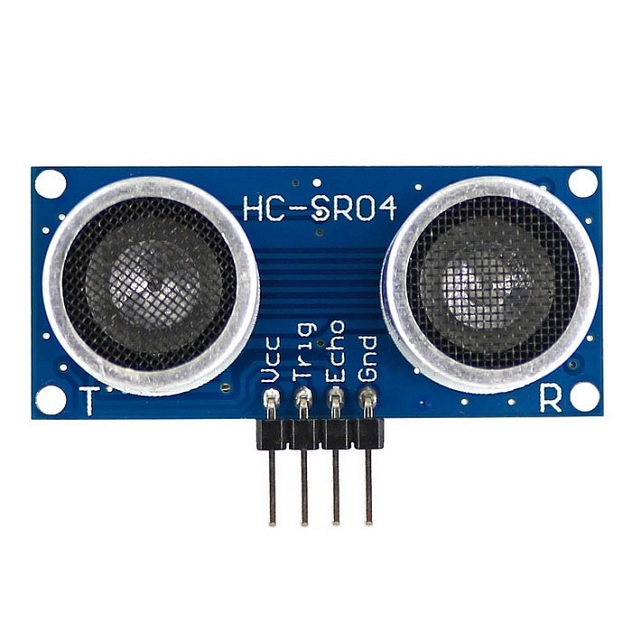
\includegraphics[width=3.5cm]{Figuras/ultrassom.jpg}
    \label{figura:ultrassom.jpeg}
    \end{figure}
    
    O funcionamento do sensor é muito simples, o que muitos podem ter achado se tratar de duas câmeras na verdade são um alto-falante e um microfone. O alto-falante emite uma onda sonora de alta frequência, altas demais para que nós humanos sejamos capazes de escutá-la, essa onda de som é refletida assim que ela vai de encontro a algum objeto e retorna para o microfone.
    
    \textit{Mas qual a utilidade em você emitir um som e depois escutá-lo de volta?}
    
    A funcionalidade não está no som em sí, mas sim no tempo que demorou para que a onda sonora retornasse para o sensor, essa informação de tempo é então utilizada para calcular a distância do sensor até o objeto que refletiu a onda de volta.
    
    O sensor ultrassônico é utilizado para obtermos a distância entre o robô e algum objeto à sua frente, mas claro que nem sempre conseguimos encontrar essa distância como esperado, isso porque tem hora que o objeto não está bem posicionado e ai ele não reflete o som de volta para o microfone, ou então ele absorve todo o som, isso pode acontecer se ele for muito macio.
    
    \begin{figure}[h]
    \caption{O objeto tem que se capaz de refletir a onda de volta para o microfone}
     
    \centering 
    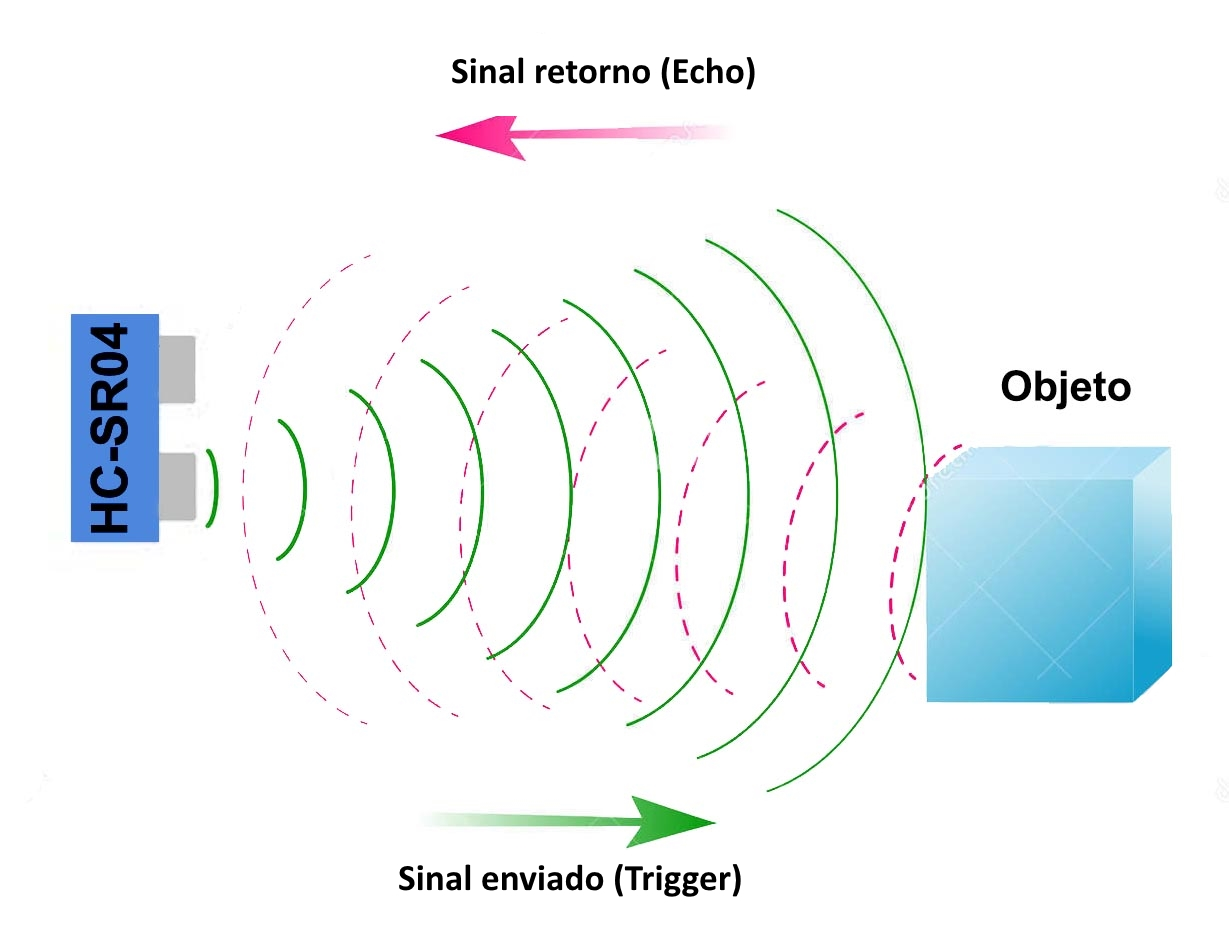
\includegraphics[width=7cm]{Figuras/onda.jpg}
    \label{figura:onda.jpeg}
    \end{figure}
    
\section{Aplicações no Cotidiano}

    \subsection*{Ultrassonografia}
        A ultrassonografia, também conhecida por ecografia e ultrassom, é um exame de diagnóstico que serve para visualizar em tempo real qualquer órgão ou tecido do corpo, um uso bastante comum é para observar o desenvolvimento do feto durante a gravidez, aquelas imagens cinzas borradas que ninguém é capaz de compreender nada senão o médico são feitas utilizando o ultrassom.
        
    \subsection*{Ecolocalização}
        Embora não seja utilizada por pessoas normais, a ecolocalização ou biossonar é muito importante na vida de diversos animais como morcegos, golfinhos de baleias, eles são seres capazes de emitir ondas de alta frequência e cronometrar o tempo levado até que eles consigam escutar o seu eco, assim são capazes de conhecer seus arredores mesmo sem a necessidade da visão.
        
    \subsection*{Sonares}
        Sonares são muito utilizados por navios e submarinos para detectar a presença de outros corpos debaixo da água, seu funcionamento é idêntico ao de um biossonar utilizado por uma baleia, por exemplo. Sonares diferem dos radares pois os radares utilizam ondas de rádio para medir a distância.
        
\section{Função}

    Para podermos utilizar o sensor ultrassônico presente no \textit{Sparki} tudo o que precisamos fazer é escrever a função \mintinline{cpp}{sparki.ping()} que ela ativará o sensor. Como já dito, o sensor serve para medir a distância, logo quando ativamos ele espera-se que a gente receba algum valor de volta que indique qual é essa distância, a função \mintinline{cpp}{sparki.ping()} então também já faz os cálculos necessários e \textbf{retorna} para a gente o valor da distância em \textbf{centímetros}.
    \\~\\
    \textit{A função então nos devolve um valor, mas como que eu vejo isso? Onde que ele vai me falar qual a distância que ele mediu? Ele escreve em algum lugar?}
    \\~\\
    AHA! Acabamos de chegar na parte importante desse capítulo, as funções que retornam valores. O \textit{Sparki} irá escrever o valor que o sensor encontrou no local que a gente determinar para isso, mas claro que isso não quer dizer que podemos simplesmente falar para ele escrever a resposta num papel que ele irá fazer (possível, mas o código para isso seria muito grande). Nós é que criamos o local onde ele deve escrever a resposta, mas esse local não pode ser qualquer um, ele tem que ser uma \textbf{variável}, e sempre que criamos uma variável temos que definir também o tipo dela, e como no nosso caso estamos trabalhando apenas com centímetros é mais adequado criar uma variável \textbf{inteira}.
    
    O código que mostra como fazemos isso está escrito logo abaixo:
    
    \begin{minted}{cpp}
    #include <Sparki.h>
    int distancia_em_cm;
    void setup()
    {
    }
    void loop()
    {
    distancia_em_cm = sparki.ping();  
    delay(300);
    }
    \end{minted}
    
    Nesse código estamos dizendo que o \textit{Sparki} deve executar a função \mintinline{cpp}{sparki.ping()} e salvar o valor que ela retornar dentro da nossa variável \textit{distancia\underline{\hspace{.1in}}em\underline{\hspace{.1in}}cm}. Agora que temos a nossa distância salva dentro de uma variável, podemos trabalhar com ela livremente para fazermos o que quiser, como fazer ele escrever o valor numa folha de papel.
    
    É importante notar a presença da função \mintinline{cpp}{delay()} no código, isso porque o funcionamento do sensor não é tão rápido quanto a velocidade de processamento do nosso robô, então precisamos dar um pequeno intervalo de tempo para que o sensor possa funcionar sem erros.
    
\section{Servo motor}
    
    Se considerarmos o sensor ultrassônico como sendo a cabeça do robô, é muito útil que tenhamos também um pescoço que sirva para movimentarmos nossa cabeça, e é ai que entra um outro servo motor presente no \textit{Sparki}. Você deve se lembrar da \textbf{garra} apresentada no capítulo de movimentação, assim como o nosso "pescoço", a garra também funciona por meio da ação de um servo motor, mas afinal o que ele é?
    
    \begin{figure}[h]
    \caption{Imagem de um servo motor}
    
    \centering 
    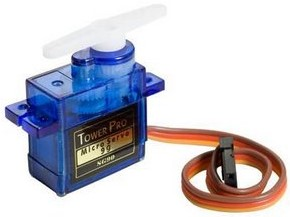
\includegraphics[width=7cm]{Figuras/servo.jpg}
    \label{figura:servo.jpeg}
    \end{figure}
    
    Um servo motor é um motor que tem a capacidade de girar o seu eixo em ângulos precisos até 90º ou 180º normalmente, sendo que o servo motor no qual o sensor ultrassônico está acoplado é capaz de girar seu eixo em até 180º. Ele é muito útil para movimentar braços robóticos por exemplo, onde não é necessário a realização de voltas completas e a precisão é importante. No nosso caso, utilizamos dele para girar o sensor e assim podermos medir distâncias em outras direções sem ter que utilizar das rodas para girar o robô, infelizmente não temos como fazer o \textit{Sparki} olhar para cima ou para baixo utilizando de um servo motor apenas.
    
\subsection{Função}

    Agora que sabemos da existência do servo motor precisamos saber como utilizamos ele, para ativá-lo escrevemos a função \mintinline{cpp}{sparki.servo()}, esta função deve receber um valor de angulação em graus que deve ser quanto que ele deve girar, este valor deve estar entre -90º e 90º (sendo valores negativos para a esquerda e positivos para a direita) e o valor pode ser um número quebrado, isto é, o argumento da função é do tipo \textbf{float}.
    
    Para facilitar a nossa vida, a função \mintinline{cpp}{sparki.servo()} já vem com 3 valores predefinidos dos ângulos mais utilizados: SERVO\underline{\hspace{.1in}}LEFT (-90º),  SERVO\underline{\hspace{.1in}}CENTER (0º) e SERVO\underline{\hspace{.1in}}RIGHT (90º), assim tudo o que precisamos fazer é escrever SERVO\underline{\hspace{.1in}}| com o sentido desejado como argumento que o \textit{Sparki} se encarrega de colocar o sensor na posição correta.
    \\~\\
    Abaixo temos um código que faz com que o \textit{Sparki} meça a distância dele para os objetos na sua esquerda, frente, direita e diagonais esquerda e direita.
    \begin{minted}{cpp}
    #include <Sparki.h>
    int distancia_esquerda, distancia_direita, distancia_frente,
    distancia_diagonal_esquerda, distancia_diagonal_direita;
    void setup()
    {
    sparki.servo(SERVO_LEFT);                    //gira para a posição -90º
    delay(500)
    distancia_esquerda = sparki.ping();  
    delay(500);
    sparki.servo(-45);                           //gira para a posição -45º
    delay(500)
    distancia_diagonal_esquerda = sparki.ping();  
    delay(500);
    sparki.servo(SERVO_CENTER);                  //gira para a posição 0º
    delay(500)
    distancia_frente = sparki.ping();  
    delay(500);
    sparki.servo(45);                            //gira para a posição 45º
    delay(500)
    distancia_diagonal_direita = sparki.ping();  
    delay(500);
    sparki.servo(SERVO_RIGHT);                   //gira para a posição 90º
    delay(500)
    distancia_direita = sparki.ping();  
    delay(500);
    }
    void loop()
    {
    }
    \end{minted}    
    

\section{Exercícios}

    \question{Responda a seguinte pergunta: como que podemos encontrar a medida de distância até um objeto utilizando apenas a informação de tempo que a onda de alta frequência demorou para retornar ao sensor?}

    \question{Com os conhecimentos adquiridos até agora, escreva um pequeno código que mostre a todo momento na tela LCD a distância do \textit{Sparki} até algum objeto que esteja na sua frente.}

    
    \question{Escreva um código que centre o sensor ultrassônico quando o \textit{Sparki} é ligado e que depois de 3 segundos faça ele ficar balançando o sensor de um lado para o outro.}
    
    \question{Escreva um código que faça com que o \textit{Sparki} determine a distância até o objeto logo a sua frente e então ande na direção dele e pare a 7cm de distância do objeto.}


    \challenge{\large{Desafio: Escreva um código onde o \textit{Sparki} gira em até 360º e então mostra na tela LCD as distâncias dos objetos a sua volta nas direções norte, nordeste, leste, sudeste, sul, sudoeste, oeste e noroeste.}}
\chapter{Variáveis}
\section*{Introdução}
    Neste capítulo, iremos abordar um dos conceitos mais importantes para nós: o que são variáveis e o que elas fazem?
\section{Variável}
    Provavelmente você já ouviu o seu professor de matemática ou de física falando dessa tal de variável e você também usou muitas variáveis enquanto estudava, mas o que na verdade é essa tal de variável? \par
    Existem várias maneiras de definir o que é uma variável, por exemplo, quando seu professor de matemática falou que ela era aquela letrinha ``x'' que vinha acompanhada de uma função e que, de fato, varia com o valor de entrada desta função. No nosso caso, vamos olhar para as variáveis de uma maneira um pouquinho diferente. \par
    Pense em um armário bem organizado, em que todas as roupas são separadas de acordo com o seu tipo, por exemplo, camisas em uma gaveta, calças e shorts em outras e assim por diante. Cada divisória do armário, ou seja, cada gaveta, deverá conter apenas um tipo de roupa específico para que o armário continue organizado. 
    \textit{Pensei! Mas o que isso tem a ver com o conceito de variáveis?}
    Tem tudo a ver! Assim como cada gaveta guarda um tipo específico de roupa, cada variável guarda um tipo específico de números ou caracteres, dentre eles: números inteiros, números reais, letras,...
    
\section{Tipagem}

\section{Operações entre variáveis}

\section{Exercícios}

\question{}

\question{}

\question{}

\question{}

\question{}

\challenge{\large{Desafio:}}
\chapter{\textit{If e else}}
\section*{Introdução}
    Neste capítulo aprofundaremos nosso estudo de programação por meio de comandos que permitem a tomada de decisão, ou seja,  estruturas auxiliares que estabelecem uma condição para a execução de um comando principal. \textsl{Ficou confuso? Não se preocupe, vou explicar a seguir!}

\section{Estruturas de decisão}
    Desde o momento em que acordamos, estamos tomando decisões, às vezes até sem perceber! Por exemplo, optar por ficar alguns minutos a mais na cama e adiar o despertador ou decidir levantar no instante em que ele tocar. Vamos supor que amanhã você tem uma prova muito importante às 8 horas da manhã, o fato de escolher ignorar o despertador e dormir mais pode resultar em consequências, como perder aquela prova de final de semestre e, possivelmente, acabar ficando com nota baixa. Como não é isso que queremos, é sempre bom acordar cedo em dias que tivermos provas pela manhã.
    
    \begin{center}
        \textsl{Estabelecemos uma condição para acordar cedo, você percebeu? A condição de acordar cedo é se houver uma prova pela manhã... É exatamente isso que faremos neste capítulo! Estabeleceremos condições para que o \textsl{Sparki} realize determinada ação!}
    \end{center}
   
    \indent As estruturas de decisão que utilizaremos são ``if'' e ``else'', elas significam ``se'' e ``senão'' em inglês, respectivamente.
    
\section{Como utilizar ``if'' e else''?}
    A seguir temos exemplos de uso dessas estruturas:
    \\
    \\
    \textsc{Exemplo 1)} Exemplo base. (Apenas para fins didáticos)
    \\
    \\
    \noindent \mintinline{cpp}{if}(Condição 1) \{\\
    \indent Ação 1;\\
    \} \mintinline{cpp}{else} \{\\
    \indent Ação 2;\\
    \}\\
    
    Esse exemplo significa que, se a ``Condição 1'' for verdadeira, o Sparki\textsl{Sparki} executará a ``Ação 1'', senão, ele executará a ``Ação 2''. Utilizar o \mintinline{cpp}{else} como uma opção alternativa ao \mintinline{cpp}{if()} é optativo, ou seja, podem existir expressões condicionais apenas com \mintinline{cpp}{if()}.
    
    \begin{center}
    {\large{Reflita}}: A ``Ação 1'' e a ``Ação 2'' poderiam ser executadas sequencialmente, em apenas uma leitura desse código ?
    \end{center}
    
    A seguir temos uma tabela com todas as opções de execução do código desse primeiro exemplo: (Tente entender a tabela, apenas decorar pode te deixar confuso mais para frente)
    
    \begin{center}
    \begin{tabular}{|c|c|c|}
    \hline
    Condição 1 & Ação 1 & Ação 2 \\ \hline
    Verdadeira & Executa & Não executa \\ \hline
    Falsa & Não executa & Executa \\ \hline
    \end{tabular}
    \end{center}
    
    \textsc{Exemplo 2)} Exemplo da explicação. (Apenas para fins didáticos)
    \\
    \\
    \noindent \mintinline{cpp}{if}(For dia de prova) \{\\
    \indent Acordar mais cedo;\\
    \} \mintinline{cpp}{else} \{\\
    \indent Acordar no horário normal;\\
    \}\\
    
    Neste caso, se for o dia da prova, devemos acordar mais cedo e, se não for o dia da prova, devemos acordar no horário normal. A segunda ação apenas ocorre se a primeira não ocorrer, logo, essas duas ações não poderiam ser executadas sequencialmente, ou seja, em uma mesma verificação da condição de ser ou não dia de prova.\\
    
    \textsc{Exemplo 3)} Exemplo com ``else if''. (Apenas para fins didáticos)
    \\
    \\
    \noindent \mintinline{cpp}{if}(Condição 1) \{\\
    \indent Ação 1;\\
    \} \mintinline{cpp}{else if}(Condição 2) \{ \\
    \indent Ação 2;\\
    \} \mintinline{cpp}{else} \{\\
    \indent Ação 3;\\
    \}\\
    
    \textit{Agora apareceram \mintinline{cpp}{else} e \mintinline{cpp}{if} em uma mesma linha, o que isso significa?} \\
    Para entender os dois termos juntos, vamos revisar o significado deles separados. \mintinline{cpp}{else} significa: ``se as condições anteriores forem falsas, executar o comando dentro das chaves''. \mintinline{cpp}{if()} significa: ``se a condição dentro dos parênteses for verdadeira, executar o comando dentro das chaves''. Consequentemente, a expressão \mintinline{cpp}{else if()} implica na execução do comando apenas se as condições anteriores forem falsas e a condição dentro do parênteses for verdadeira.
    
    \begin{center}
    \begin{tabular}{|c|c|c|c|c|}
    \hline
    Condição 1 & Ação 1 & Condição 2 & Ação 2 & Ação 3\\ \hline
    Verdadeira & Executa & Falsa & Não executa & Não executa \\ \hline
    Verdadeira & Executa & Verdadeira & Não executa & Não executa \\ \hline
    Falsa & Não executa & Verdadeira & Executa & Não executa \\ \hline
    Falsa & Não executa & Falsa & Não executa & Executa \\ \hline
    \end{tabular}
    \end{center}
    
    \textsc{Exemplo 4)} Imagine uma situação hipotética em que existam 3 compromissos na sua agenda, no mesmo dia e horário, e você terá que escolher apenas um, de acordo com a previsão do tempo. (Apenas para fins didáticos)
    \\
    \\
    \noindent \mintinline{cpp}{if}(Estiver fazendo muito calor) \{ \\
    \indent Ir ao clube; \\
    \} \mintinline{cpp}{else if}(Estiver chovendo) \{ \\
    \indent Ver um filme em casa;\\
    \} \mintinline{cpp}{else if}(Estiver nevando) \{ \\
    \indent Ir esquiar;\\
    \} \mintinline{cpp}{else} \{ \\
    \indent Ir ao cinema.\\
    \}\\
    
    \textit{Isshh... Agora ficou complicado! E se a previsão do tempo afirmar que vai chover e nevar nesse dia? Qual compromisso eu escolho?} 
    \\
    Essa é fácil! É necessário apenas observar qual das condições será lida primeiro nesse código, ou seja, o que vier primeiro! Como a condição ``Estiver chovendo'' aparece primeiro, o compromisso seria ``Ver um filme em casa''.
    
    \textit{E qual seria a condição para ``Ir ao cinema''?} 
    \\
    A condição seria a negação das anteriores, neste caso, se não estivesse fazendo muito calor, nem chovendo, nem nevando.
    
    Uma curiosidade dessa estrutura condicional é que se escrevermos ``1'' dentro dos parênteses do \mintinline{cpp}{if()}, ele será verdadeiro e o que estiver dentro das chaves será executado. Assim, se escrevermos ``0'' dentro dos parênteses, o \mintinline{cpp}{if()} será falso e o que estiver dentro das chaves não será executado. Isso se dá porque a programação possui uma base binária, ou seja, ela é baseada em vários ``1'' e ``0''.
    
    \section{Operações de comparação}
    
    Iremos aprender nesta seção os tipos de operadores que podemos utilizar para comparar dois valores ou incógnitas. Lembrando que eles devem ser utilizados apenas dentro do parênteses do \mintinline{cpp}{if()}. São eles:
    
    \begin{itemize}
        \item ``=='' para verificar se os dois valores são iguais.
        \item ``!='' para verificar se os dois valores são diferentes.
        \item ``>'' para verificar se o primeiro é maior que o segundo.
        \item ``>='' para verificar se o primeiro é maior que o segundo ou igual a ele.
        \item ``<'' para verificar se o primeiro é menor que o segundo.
        \item ``<='' para verificar se o primeiro é menor que o segundo ou igual a ele.
    \end{itemize}
    
    Agora que você já entendeu como funcionam as expressões condicionais e os operadores de comparação, vamos para um exemplo de verdade!
    \\
    \\
    \textsc{Exemplo 1)} Atribuiremos o valor 2042385 à variável x e queremos que o \textsl{Sparki} responda se esse número é ímpar ou par. Para isso, utilizaremos a informação da sessão anterior sobre os ``1'' e os ``0''.
    
    \begin{minted}{cpp}
    #include <Sparki.h>
    void setup()
    {
        int x = 2042385;
    }
    void loop()
    {
        sparki.clearLCD();
        if(x % 2) {
            sparki.print("O numero e impar.");
        } else {
            sparki.print("O numero e par.");
        }
        sparki.updateLCD();
        delay(1000);
    }
    \end{minted}
    
    Sabemos que o número 2042385 é ímpar pela regra da divisão por 2, que afirma que um número é divisível por 2 quando o último algarismo dele for divisível por 2. Nesse código, não utilizamos essa regrinha, mas sim o método mais tradicional, fazemos o \textsl{Sparki} verificar se a divisão desse número por 2 é exata, ou seja, se o resto é 0. Assim, o \textsl{Sparki} chega a mesma conclusão que chegamos, que o número 2042381 é ímpar, e imprime essa informação no LCD.
    
    \begin{center}
    \textcolor{teal}{Lembrando:}
    O símbolo ``\%'' significa o resto da divisão do primeiro número pelo segundo.
    \end{center}
    
    \textsc{Exemplo 2)} Dessa vez, faremos com que o \textsl{Sparki} responda se o número 2042385 é divisível por 3 e por 5.
    
    \begin{minted}{cpp}
    #include <Sparki.h>
    void setup()
    {
        int x = 2042385;
    }
    void loop()
    {
        sparki.clearLCD();
        if((x % 3) == 0) {
            sparki.println("O numero e divisivel por 3.");
        } else {
            sparki.println("O numero nao e divisivel por 3.");
        }
        if((x % 5) == 0) {
            sparki.print("O numero e divisivel por 5.");
        } else {
            sparki.print("O numero nao e divisivel por 5.");
        }
        sparki.updateLCD();
        delay(1000);
    }
    \end{minted}
    
    Esse exemplo é parecido com o anterior, mas ele está aqui para mostrar que podemos inserir duas estruturas condicionais independentes em um mesmo código. As duas comparações para saber se o número é divisível por 3 e por 5 não dependem uma da outra, pois um número pode ser divisível por 3 e por 5 ao mesmo tempo, por isso que existem dois \mintinline{cpp}{if()} e dois \mintinline{cpp}{else}. Consequentemente, o \textsl{Sparki} imprimirá duas mensagens na tela, na primeira linha: ``O numero e divisivel por 3'' e na segunda: ``O numero e divisivel por 5''.
    
    \textsc{Exemplo 3)} Exemplo de comparação de variáveis.
    
    \begin{minted}{cpp}
    #include <Sparki.h>
    void setup()
    {
        int x = 10;
        int y = 100;
    }
    void loop()
    {
        sparki.clearLCD();
        if(x >= y) {
            sparki.print("Condicao 1");
        } else if(y != (x * x)) {
            sparki.print("Condicao 2");
        } else if((y / x) >= x) {
            sparki.print("Condicao 3");
        } else if((y - 100) <= x){
            sparki.print("Condicao 4");
        }
        sparki.updateLCD();
        delay(1000);
    }
    \end{minted}
    
    Então, já sabe o que o \textsl{Sparki} fará ao ler este código? Vamos ver passo a passo:
    
    \begin{itemize}
        \item[Condição 1)]
        \begin{eqnarray}
        x & == & y\\
        10 & == & 100 \nonumber     \end{eqnarray}
        Essa afirmação é FALSA, logo, o \textsl{Sparki} não executará a ação entre as chaves.
        \item[Condição 2)]
        \begin{eqnarray}
        y & != & (x * x)\\
        100 & != & 10 * 10 \nonumber\\
        100 & != & 100 \nonumber
        \end{eqnarray}
        Essa afirmação também é FALSA, por isso a ação não será executada.
        \item[Condição 3)]
        \begin{eqnarray}
        (y / x) & >= & x\\
        (100 / 10) & >= & 10 \nonumber\\
        10 & >= & 10 \nonumber\\
        \end{eqnarray}
        Essa afirmação é verdadeira, logo, o \textsl{Sparki} executará a ação entre as chaves, imprimirá no LCD ``Condicao 3''.
        \item[Condição 4)]
        Essa condição não será nem lida, pois ela só poderia ser executada se todos os \mintinline{cpp}{if()} anteriores, dentro dessa estrutura condicional, fossem falsos.
    \end{itemize}
    
    \begin{center}
    \textcolor{teal}{Lembrando:}
    Sempre devemos executar a operação dentro dos parênteses antes dos operadores de comparação.
    \end{center}

\section{Fluxograma ou Diagrama de Fluxo}

    \begin{center}
    \textbf{Definição} 
    \\
    Uma representação gráfica de passos sequenciais e decisões a serem tomadas durante a execução de um processo.
    \end{center}
    
    Esboçar um Fluxograma antes de programar pode ser muito útil, principalmente quando se está aprendendo ainda. Dentre as principais vantagens de se fazer um Fluxograma, temos:
    \begin{itemize}
        \item Poder escolher a melhor solução para o problema;
        \item Organizar as ideias antes de começar a programar de fato;
        \item Evitar erros de lógica.
    \end{itemize}

    Por ser um representação gráfica de um programa, iremos aprender símbolos para cada tipo de execução, como, por exemplo, o início e o fim do programa, as entradas de informação, as ações do \textsl{Sparki}, as tomadas de decisão e o fluxo de informações. A figura a seguir mostra os símbolos gráficos correspondentes a cada um dos exemplos citados:
    
    \begin{figure}[h]
    \caption{Símbolos de um Fluxograma.}
     
    \centering 
    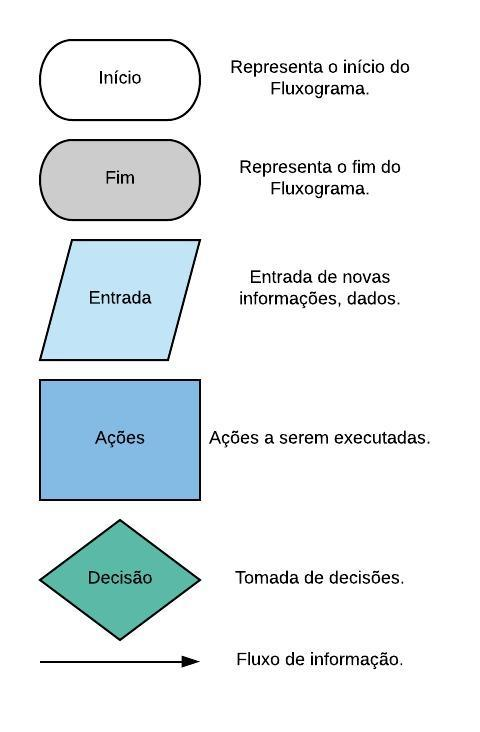
\includegraphics[width=5cm]{Figuras/Diagrama em branco.jpeg}
    \label{figura:Diagrama em branco.jpeg}
    \end{figure}
 
\section{Operadores lógicos}
    Nesta seção, iremos aprender a lidar com comparações que envolvem mais de um fator a ser analisado e, para isso, utilizaremos o início da teoria da Álgebra Booleana, criada por George Boole. 
 
     Na Álgebra de Boole, existem 3 tipos de operadores lógicos: E, OU e NÃO, cada um com uma funcionalidade própria. Eles devem ser usados dentro de condicionais \mintinline{cpp}{if()} para ligar duas comparações ou para negar uma ou mais comparações.
 
\subsection{E (AND)}
 
    Este operador depende de pelo menos dois ``resultados'' de afirmações, por exemplo, vamos supor que você quer ir à piscina, mas você apenas irá se estiver fazendo sol \textbf{E} se a piscina estiver limpa. Então, a 1ª afirmação é: se estiver fazendo sol e a 2ª afirmação é: se a piscina estiver limpa. O operador AND vai funcionar como uma ``ponte'' de ligação entre essas duas afirmações. 
    
    \begin{center}
        A condição estabelecida pelo \mintinline{cpp}{if()}, com o AND entre as afirmações, será VERDADEIRA apenas quando as afirmações forem ambas VERDADEIRAS.
    \end{center}
    
    \textit{Então o AND vai ser uma comparação entre duas comparações?? Que confuso!}
    
    Mais ou menos... É mais certo dizer que o AND irá realizar uma operação entre as duas comparações/afirmações. Utilizando o exemplo anterior, as duas afirmações têm que ser verdadeiras, ou seja, 1) tem que estar fazendo sol e 2) a piscina tem que estar limpa para que a comparação seja verdadeira e você possa ir à piscina.
    \\
    \\
    \textsc{Exemplo 0)} Exemplo da explicação, apenas para fins didáticos.
    \\
    \\
    \mintinline{cpp}{if}(Fizer sol AND Piscina estiver limpa) \{\\
    \indent Ir à piscina;\\
    \} \mintinline{cpp}{else} \{\\
    \indent Não ir à piscina;\\
    \}
    
    Se a comparação 1 der VERDADEIRA e a comparação 2 der FALSA, o \mintinline{cpp}{if()} não será realizado e você não irá à piscina. Porém, se as duas comparações derem VERDADEIRAS, o \mintinline{cpp}{if()} será realizado e você poderá ir à piscina.
    
    Agora, vamos fazer um esquema com todas as possibilidades de combinação entre duas comparações e ver o resultado final:
    
    \begin{itemize}
        \item VERDADEIRO AND VERDADEIRO -> Resultado: VERDADEIRO
        \item VERDADEIRO AND FALSO -> Resultado: FALSO
        \item FALSO AND VERDADEIRO -> Resultado: FALSO
        \item FALSO AND FALSO -> Resultado: FALSO
    \end{itemize}
    
    \begin{center}
    \textcolor{teal}{Lembrando:}
    Resultado: VERDADEIRO, significa que o \mintinline{cpp}{if()} será executado. 
    Resultado: FALSO, significa que o \mintinline{cpp}{if()} não será executado.
    \end{center}
 
    \textit{Tá, mas como eu aplico isso na programação?}
        
    Na programação, utilizamos os caracteres ``\&\&'' para simbolizar o AND. Aqui temos um exemplo:
    \\
    \\
    \textsc{Exemplo 1)} Neste exemplo, serão criadas 3 variáveis para armazenar a idade de 3 crianças: o Enzo, que tem 1 ano, a Valentina, que tem 2 anos, e a Sofia com 3 anos. Se a idade das 3 crianças forem iguais, o \textsl{Sparki} andará para frente, se a Sofia for a mais velha e o Enzo o mais novo, o \textsl{Sparki} andará para trás, e, por último, se as duas condições anteriores forem falsas, o \textsl{Sparki} ficará parado.

    \begin{minted}{cpp}
    #include <Sparki.h>
    void setup()
    {
    int idade_enzo = 1;
    int idade_valentina = 2;
    int idade_sofia = 3;
    }
    void loop()
    {
        if(idade_enzo == idade_valentina && idade_enzo != idade_sofia){
            //Se o Enzo e a Valentina tiverem a mesma idade e a Sofia tiver uma idade diferente
            //Neste caso, FALSO AND VERDADEIRO -> Resultado: FALSO
            sparki.moveForward();
        } else if(idade_valentina > idade_enzo && idade_sofia > idade_valentina) {
            //Se o primeiro caso for falso e a Sofia for mais velha que a Valentina, que for mais velha que o Enzo
            //Neste caso, VERDADEIRO AND VERDADEIRO -> Resultado: VERDADEIRO
            sparki.moveBackward();
        } else {
            //Se o primeiro e o segundo caso forem falsos
        }
    }
    \end{minted}
    
    O \textsl{Sparki} andará para trás.
    \begin{itemize}
        \item[Condição 1)]
        \begin{eqnarray}
        idade\_enzo & = & idade\_valentina\\
        1 & = & 2 \nonumber     \end{eqnarray}
        Essa afirmação é FALSA.
        \begin{eqnarray}
        idade\_enzo & != & idade\_sofia\\
        1 & != & 3 \nonumber
        \end{eqnarray}
        Essa afirmação é VERDADEIRA.
        Como temos o ``\&\&'' (AND) ligando as duas afirmações, a comparação será FALSA.
        \item[Condição 2)]
        \begin{eqnarray}
        idade\_valentina & > & idade\_enzo
        \end{eqnarray}
        Essa afirmação é VERDADEIRA.
        \begin{eqnarray}
        idade\_sofia & > & idade\_valentina
        \end{eqnarray}
        Essa afirmação também é VERDADEIRA. Como as duas afirmações são verdadeiras e o ``\&\&'' (AND) está ligando-as, a comparação será VERDADEIRA.
    \end{itemize} 
    
    \textsc{Exemplo 2)} Um exemplo com as mesmas variáveis anteriores, mas um pouco mais complicado.
    
    \begin{minted}{cpp}
    #include <Sparki.h>
    void setup()
    {
    int idade_enzo = 1;
    int idade_valentina = 2;
    int idade_sofia = 3;
    }
    void loop()
    {
        sparki.clearLCD();
        if((idade_sofia - idade_valentina) == idade_enzo && (idade_valentina - idade_enzo) == 3) {
            //VERDADEIRO AND FALSO -> Resultado: FALSO
            sparki.drawCircleFilled(63, 32, 10);
        } else if((idade_enzo + 1) != 2 && (idade_valentina - idade_enzo) != idade_sofia) {
            //FALSO AND VERDADEIRO -> Resultado: FALSO
            sparki.drawRectFilled(10,0, 15, 30);
        } else if((idade_enzo * 6) == (idade_valentina * 3)) {
            //VERDADEIRO
            sparki.drawChar(10, 1, 'a');
        } else {
            sparki.drawString(40, 4, "123");
        } 
        sparki.updateLCD();
        delay(1000);
    }
    \end{minted}
    
    O \textsl{Sparki} irá imprimir o caracter ``a'' no LCD.
    \begin{itemize}
        \item[Condição 1)]
        \begin{eqnarray}
        (idade\_sofia - idade\_valentina) & = & idade\_enzo\\
        (3 - 2) & = & 1 \nonumber \\
        1 & = & 1 \nonumber
        \end{eqnarray}
        Essa afirmação é VERDADEIRA.
        \begin{eqnarray}
        (idade\_valentina - idade\_enzo) & = & 3\\
        (2 - 1) & = & 3 \nonumber \\
        1 & = & 3 \nonumber
        \end{eqnarray}
        Essa afirmação é FALSA.
        Como temos o ``\&\&'' (AND) ligando essas duas afirmações, a comparação será FALSA.
        \item[Condição 2)] 
        \begin{eqnarray}
        (idade\_enzo + 1) & != & 2\\
        (1 + 1) & != & 2 \nonumber \\
        2 & != & 2 \nonumber
        \end{eqnarray}
        Essa afirmação é FALSA.
        \begin{eqnarray}
        (idade\_valentina - idade\_enzo) & != & idade\_sofia)\\
        (2 - 1) & != & 3 \nonumber \\
        1 & != & 3 \nonumber
        \end{eqnarray}
        Essa afirmação é VERDADEIRA. Como o ``\&\&'' (AND) está ligando essas duas afirmações, a comparação será FALSA
        \item[Condição 3)] 
        \begin{eqnarray}
        (idade\_enzo * 6) & = & (idade\_valentina * 3)\\
        (1 * 6) & = & (2 * 3) \nonumber \\
        6 & = & 6 \nonumber 
        \end{eqnarray}
        Essa afirmação é VERDADEIRA, logo, a comparação também é.
    \end{itemize}
    
    \begin{center}
    \textcolor{cyan}{Para não esquecer!}
    \\``And'' traduzido para o português significa ``e''.
    \end{center}
     
\subsection{OU (OR)}
    Este operador deve ser colocado entre duas ou mais afirmações, assim como o AND. Vamos supor que a sua mãe está viajando e você combinou de se encontrar com ela quando ela chegasse no aeroporto. O combinado foi o seguinte: ela mandaria mensagem \textbf{OU} ligaria quando estivesse embarcando no voo de volta, e você sairia de casa por volta de 30 minutos depois, para se encontrar com ela no aeroporto.
    
    \begin{center}
        A condição estabelecida pelo \mintinline{cpp}{if()}, com o OR entre as afirmações, será VERDADEIRA se pelo menos uma das duas comparações forem VERDADEIRAS.
    \end{center}
   
    \textsc{Exemplo 0)} Exemplo da explicação, apenas para fins didáticos.
    \\
    \\
    \mintinline{cpp}{if}(Sua mãe te mandasse mensagem OR Sua mãe te ligasse) \{\\
    \indent Esperar 30 minutos;\\
    \indent Sair de casa;\\
    \} \mintinline{cpp}{else} \{\\
    \indent Continuar esperando a mensagem ou a ligação;\\
    \}
     
     Então, se a sua mãe te ligasse (afirmação VERDADEIRA) mas não te mandasse mensagem (afirmação FALSA), a condição do \mintinline{cpp}{if()} seria VERDADEIRA e você esperaria 30 minutos para sair de casa. Se as duas afirmações foram VERDADEIRAS, ou seja, se ela te mandar mensagem e te ligar, a condição \mintinline{cpp}{if()} também será VERDADEIRA, neste caso, você também executará as ações dentro das chaves do \mintinline{cpp}{if()}.
     A seguir temos todos os resultados possíveis para um OR entre duas afirmações:
     
     \begin{itemize}
        \item VERDADEIRO OR VERDADEIRO -> Resultado: VERDADEIRO
        \item VERDADEIRO OR FALSO -> Resultado: VERDADEIRO
        \item FALSO OR VERDADEIRO -> Resultado: VERDADEIRO
        \item FALSO OR FALSO -> Resultado: FALSO
    \end{itemize}
    
    Na programação, utilizamos os caracteres ``||'' para simbolizar o OR.
    \\
    \\
    \textsc{Exemplo 1)}
     
     \begin{minted}{cpp}
    #include <Sparki.h>
    void setup()
    {
    int idade_enzo = 1;
    int idade_valentina = 2;
    int idade_sofia = 3;
    }
    void loop()
    {
        if(idade_enzo == idade_valentina || idade_sofia != idade_ valentina) {
        //Neste caso, FALSO OR VERDADEIRO -> Resultado: VERDADEIRO
        sparki.moveBackward();
        } else if(idade_valentina ==  (idade_sofia - 1) || (idade_valentina + 1) == idade_sofia) {
        //Neste caso, VERDADEIRO OR VERDADEIRO -> Resultado: VERDADEIRO
        sparki.moveForward();
        } else {
        //Se a primeira e a segunda condição forem falsas
        sparki.moveRight();
        }
    }
    \end{minted}
    
    O \textsl{Sparki} andará para trás.
    \begin{itemize}
        \item[Condição 1)] 
        \begin{eqnarray}
        idade\_enzo & = & idade\_valentina
        \end{eqnarray}
        Essa afirmação é FALSA.
        \begin{eqnarray}
        idade\_sofia & != & idade\_valentina
        \end{eqnarray}
        Essa afirmação é VERDADEIRA. Como o ``||'' (OR) liga essas duas afirmações, sabemos que a comparação será VERDADEIRA.
        \item[Condição 2)] Essa condição não será nem lida, pois ela só poderia ser executada se todos os \mintinline{cpp}{if()} anteriores, dentro dessa estrutura condicional, fossem falsos.
    \end{itemize}

    \textsc{Exemplo 2)}
     
    \begin{minted}{cpp}
    #include <Sparki.h>
    void setup()
    {
    int idade_enzo = 1;
    int idade_valentina = 2;
    int idade_sofia = 3;
    }
    void loop()
    {
        sparki.clearLCD();
        if(idade_valentina != 2 || idade_enzo != 1) {
            //FALSO OR FALSO -> Resultado: FALSO
            sparki.print("Condicao 1");
        } else if(idade_sofia != (idade_valentina - 1) || idade_sofia == idade_enzo) {
            //VERDADEIRO OR FALSO -> Resultado: FALSO
            sparki.print("Condicao 2");
        } else if((idade_enzo + 2) == (idade_sofia + 1) ||     idade_enzo == (4 - idade_sofia)) {
            //FALSO OR VERDADEIRO -> Resultado: FALSO
            sparki.print("Condicao 3");
        } else {
            sparki.print("Nenhuma das anteriores");
        }
        sparki.updateLCD();
        delay(1000);
    }
    \end{minted}
    
    O \textsl{Sparki} irá imprimir na tela ``Nenhuma das anteriores''.
    \begin{itemize}
        \item[Condição 1)] 
        \begin{eqnarray}
        idade\_valentina != 2\\
        idade\_enzo != 1 \nonumber
        \end{eqnarray}
        Essa afirmação é FALSA.
        \item[Condição 2)]
        \begin{eqnarray}
        idade\_sofia & = & idade\_enzo;
        \end{eqnarray}
        Essa afirmação é FALSA.
        \item[Condição 3)]
        \begin{eqnarray}
        (idade\_enzo + 2) & = & (idade\_sofia + 1)\\
        (1 + 2) & = & (3 + 1) \nonumber \\
        3 & = & 4 \nonumber
        \end{eqnarray}
        Essa afirmação é FALSA.
    \end{itemize}
     
    \begin{center}
        \textcolor{cyan}{Para não esquecer!}
        \\``Or'' traduzido para o português significa ``ou''.
    \end{center}
     
\subsection{NÃO (NOT)}

    \begin{itemize}
        \item NOT(VERDADEIRO) -> Resultado: FALSO
        \item NOT(FALSO) -> Resultado: VERDADEIRO
    \end{itemize}
    
    Na programação, utilizamos o caracter ``!'' para simbolizar o NOT.
    \\
    \\
     \textsc{Exemplo 1)}
     
     \begin{minted}{cpp}
    #include <Sparki.h>
    void setup()
    {
    int idade_enzo = 1;
    int idade_valentina = 2;
    int idade_sofia = 3;
    }
    void loop()
    {
        if(!(idade_enzo == 1) {
            //NOT(VERDADEIRO) -> Resultado: FALSO
        } else if(!(idade_valentina == 3)) {
            //NOT(FALSO) -> Resultado: VERDADEIRO
            sparki.moveForward();
        } else if(!(idade_sofia != 3)) {
            //NOT(FALSO) -> Resultado: VERDADEIRO
            sparki.moveBackward();
        }
    }
    \end{minted}
    
    O \textsl{Sparki} andará para frente, pois
    \begin{itemize}
        \item[Condição 1)]
        \begin{eqnarray}
        !(idade\_enzo & = & 1)\\
        !(1 & = & 1) \nonumber         \end{eqnarray}
        Sabemos que a afirmação 1 = 1 é VERDADEIRA, mas há um caracter ``!'' antes dela, por isso, ela acaba se tornando FALSA.
        \item[Condição 2)]
        \begin{eqnarray}
        !(idade\_valentina & = & 3)\\
        !(2 & = & 3) \nonumber
        \end{eqnarray}
        A afirmação 2 = 3 é FALSA, mas o caracter ``!'' antes dela a torna VERDADEIRA.
        \item[Condição 3)] Essa condição não será lida.
    \end{itemize}
    
     \textsc{Exemplo 2)} Agora que você aprendeu todos os operadores lógicos, podemos fazer um exemplo misturando todos eles! Dessa vez vou pedir pra você tentar entender todo o código antes de ler a explicação. Vamos nessa?!
     
     \begin{minted}{cpp}
    #include <Sparki.h>
    void setup()
    {
    int x = 0;
    int y = 10;
    int z = 4;
    }
    void loop()
    {
        sparki.clearLCD();
        y = -2;
        x = y;
        if(!(x == 10)) {
            sparki.print("A"); //não printa
        } else if(y >= -3 && x == y) {
            z = 3;
            x = 1;
            sparki.print("b"); //printa
        } else if(z == 3 || x != -2) {
            z = 4;
           sparki.print("c"); //nao printa
        }
        sparki.print("D"); //printa
        x += 0;
        if(!(x == 0 || z != 3)) {
            sparki.print("E"); //printa
            sparki.print("f"); //printa
            sparki.updateLCD();
            sparki.clearLCD(); //apaga tudo
        } else {
            sparki.print("G");
        }
        sparki.updateLCD();
        sparki.print("h");
        delay(2000);
    }
    \end{minted}
     
    Entendeu tudinho? Vamos ver se você acertou o que o \textsl{Sparki} irá fazer dessa vez!
    %Falta terminar
    
    
    
    \begin{center}
        \textcolor{cyan}{Para não esquecer!}
        \\``Not'' traduzido para o português significa ``não''.
    \end{center}
 
\section{Garras e controle remoto}

\section{LCD2: fazendo uma animação na tela do Sparki}

    Agora que aprendemos o que são variáveis e estruturas de condição, podemos fazer uma animação! Mas como ainda somos iniciantes na programação, iremos começar a movimentar um objeto bem simples e conhecido na tela do \textsl{Sparki}, um círculo!\par
    Para fazer essa animação, siga os seguintes passos e vamos nessa!
    
    \begin{minted}{cpp}
    #include <Sparki.h>;
    int x = 0;
    void setup()
    {
    }
     
    void loop()
    {
        sparki.clearLCD();
        if (x < 127)
          x++;
        else
          x = 0;
        sparki.drawCircleFilled(x, 32, 10);
        sparki.updateLCD();
        delay(100);
    }
    \end{minted}

\section{Exercícios}

\question{Leia o seguinte código e marque a alternativa correspondente:}

    \begin{minted}{cpp}
    #include <Sparki.h>
    void setup()
    {
        a = 5
        b = 10
        c = a + b
    }
    void loop()
    {
        sparki.clearLCD();
        if(a != (b - 5)) {
            sparki.print("Hello World");
        } else if(a == (c - b) && b != (c - a)) {
            sparki.print("Hello");
            sparki.print("World");
        } else if(((a + 5) >= (b + 1)) || (((b + a) == c) && ((b / 2) == a))) {
            sparki.println("Hello");
            sparki.print("World");
        }
        sparki.updateLCD();
        delay(3000);
    }
    \end{minted}
    
    O que aparecerá na tela LCD do \textsl{Sparki} após 3 segundos?

    \begin{description}
    \item[a)] ``HelloWorld'' em uma linha.
    \item[b)] ``Hello'' em uma linha e ``World'' na linha de baixo.
    \item[c)] ``Hello World'' em uma linha.
    \item[d)] Nenhuma das anteriores.
    \end{description}

\question{Refaça o código do exemplo 1) da seção de ``Operações de comparação'' utilizando o operador lógico NOT.}

%Deixar espaço de linhas.

\question{}

\question{}

\question{Escreva um código para verificar se o número 34534 é divisível por 2 e 3. Se for, imprimir no LCD a mensagem ``Numero divisivel por 2 e por 3'', se não for, verificar se este número é divisível por 2 e por 3 isoladamente, com duas estruturas condicionais independentes. Se for divisível apenas por 2, imprimir no LCD ``Numero divisivel por 2'', se for divisível apenas por 3, imprimir no LCD ``Numero divisivel por 3''.}

\challenge{\large{Desafio:}Escreva um código }
\chapter{Infravermelho}

\section*{Introdução}

\section{Exercícios}

\question{}

\question{}

\question{}

\question{}

\question{}

\challenge{\large{Desafio:}}
\chapter*{Apêndice}

\chapter*{Gabarito}

\section*{Capítulo 1 - Afinal, o que é um robô?}

\section*{Capítulo 2 - Algoritmos e tela LCD}

    \subsection*{1)}
    
    \subsection*{2)}
    
    \subsection*{3)}
    
    \subsection*{4)}
    
    \subsection*{5)}
    
    \subsection*{Desafio) Perguntar ao professor.}

\section*{Capítulo 3 - Movimentação}

    \subsection*{1)}
    Letra c.
    
    \subsection*{2) (Existe mais de uma solução para este exercício)}

    \begin{minted}{cpp}
    #include <Sparki.h>
    void setup ()
    {
    }
    void loop ()
    {
        sparki.moveForward(5);
        sparki.moveRight();
    }
    \end{minted}
    
    \textsl{Como a distância a ser percorrida pelo robô é equivalente ao lado do quadrado, o valor dentro dos parênteses da função ``sparki.moveForward()'' é 5.}
    
    \subsection*{3) (Existe mais de uma solução para este exercício)} 
    
    \begin{minted}{cpp}
    #include <Sparki.h>
    void setup ()
    {
    }
    void loop ()
    {
        sparki.moveForward(500);
        sparki.moveRight();
    }
    \end{minted}
    
    \textsl{Como o lado do quadrado passou a ser 5 metros, é necessário transformar esse valor para centímetros antes de escrever dentro dos parênteses da função.}
    
    \subsection*{4)}
    Letra d.
    
    \subsection*{5)}
    %FALTA FAZER A RESPOSTA DESTE EXERCÍCIO
    
    \subsection*{Desafio) Perguntar ao professor.}
    
\section*{Capítulo 4 - Ultrassom}

    \subsection*{1)}
    
    \subsection*{2)}
    
    \subsection*{3)}
    
    \subsection*{4)}
    
    \subsection*{5)}
    
    \subsection*{Desafio) Perguntar ao professor.}

\section*{Capítulo 5 - Variáveis}

    \subsection*{1)}
    
    \subsection*{2)}
    
    \subsection*{3)}
    
    \subsection*{4)}
    
    \subsection*{5)}
    
    \subsection*{Desafio) Perguntar ao professor.}

\section{Capítulo 6 - If e Else}

    \subsection*{1)} Letra b.
    
    \subsection*{2) (Existe mais de uma solução para este exercício)}
    
    \begin{minted}{cpp}
    #include <Sparki.h>
    void setup()
    {
        int x = 2042385;
    }
    void loop()
    {
        sparki.clearLCD();
        if(!(x % 2)) {
            sparki.print("O numero e par.");
        } else {
            sparki.print("O numero e impar.");
        }
        sparki.updateLCD();
        delay(1000);
    }
    \end{minted}
    
    \subsection*{3)}
    
    \subsection*{4)}
    
    \subsection*{5)}
    
    \subsection*{Desafio) Perguntar ao professor.}

\section*{Capítulo 7 - Infravermelho}

    \subsection*{1)}
    
    \subsection*{2)}
    
    \subsection*{3)}
    
    \subsection*{4)}
    
    \subsection*{5)}
    
    \subsection*{Desafio) Perguntar ao professor.}
    
\chapter*{Dicionário}


% Referências =========================================
\bibliographystyle{abbrv} 
\bibliography{references} % nome do arquivo
\end{document}
